\vspace{5pt} \hrule \vspace{5pt}

\chapter{FEM}
\section{Sobolev空间与椭圆方程理论}

\subsection{Sobolev空间}
设$\Omega \subset \mathbb{R}^n$为带边有界连通Lipschitz区域,其中Lipschitz是说,局部上边界可以看成是Lipschitz连续函数的图像。事实上边界的光滑性都可以这么定义,只要把Lipschitz连续换成对应的光滑性。

-(根据可导性)定义$C^m(\Omega), C^m(\bar{\Omega}), C_0^m(\Omega)$,其中$C^m(\bar{\Omega})$在范数
\[
  \|u\|_{C^m(\bar{\Omega})} = \max_{|\alpha| \le m} \max_{x \in \bar{\Omega}} |\partial^\alpha u(x)|
\]
下构成Banach空间。

-(根据可积性)定义$L^p$空间$(L^p(\Omega), \|\cdot\|_{0, p, \Omega})$。($L^p$空间越来越小,尺子越来越长)$L^\infty$空间的范数为ess sup,即本性上界。

-(根据可导性和可积性)定义(正整指数)Sobolev空间$(W^{m, p}(\Omega), \|\cdot\|_{m, p, \Omega})$,$p = 2$时记为$(H^m(\Omega), \|\cdot\|_{m, \Omega})$。另外可以定义半范数$|\cdot|_{m, p, \Omega}$
\[
  \begin{aligned}
    \|u\|_{m, p, \Omega}^p = \sum_{|\alpha| \le m} \|\partial^\alpha u\|_{0, p, \Omega}^p\\
    |u|_{m, p, \Omega}^p = \sum_{|\alpha| = m} \|\partial^\alpha u\|_{0, p, \Omega}^p
  \end{aligned}
\]

另一种等价的定义是:$W^{m, p}(\Omega)/W^{m, p}_0(\Omega)$为$C^{\infty}(\Omega)/C^{\infty}_0(\Omega)$在$\|\cdot\|_{m, p, \Omega}$下的完备化空间。于是$C^{\infty}(\Omega) \overset{\text{dense}}{\hookrightarrow} W^{m, p}(\Omega), C^{\infty}_0(\Omega)\overset{\text{dense}}{\hookrightarrow} W^{m, p}_0(\Omega)$。

\subsection{嵌入定理和迹定理}

-(嵌入定理)设有界Lipschitz区域$\Omega$,则
\[
  W^{m, p}(\Omega) \hookrightarrow\left\{\begin{array}{ll}
    L^{q}(\Omega), 1 \le q \le \frac{n p}{n-m p} & \text { 当 } m<\frac{n}{p} \\
    L^{q}(\Omega), 1 \le q<\infty & \text { 当 } m=\frac{n}{p} \\
    C(\bar{\Omega}) & \text { 当 } m>\frac{n}{p}
  \end{array}\right.
\]

对于嵌入定理,回忆Sobolev空间的定义是说至多m阶导数p阶可积,用的是同一个可积性,但是这个函数本身的可积性可能不止,所以说不是“可导性换可积性”,而是去发掘这个函数原有的可积性,逻辑上肯定是要比p大,具体多少和空间维数n以及可导性m有关。事实上可以看到,m越大可积性越强,m充分大时甚至连续。

另外注意这里给出的嵌入定理对区域有更高的要求,此时的嵌入都是紧嵌入。紧嵌入即嵌入映射是紧的,映射是紧的如果把有界列映成收敛列。

-(迹定理)迹算子是有界线性算子。比较常用的就是
\[
  \operatorname{tr}: H^1(\Omega) \to L^2(\Omega), \quad \|v\|_{0, \partial \Omega} \le C \|v\|_{1, \Omega}
\]

\subsection{变分原理}

\begin{enumerate}
  \item Poisson方程的Dirichlet边值问题
  \[
    \left\{\begin{array}{ll}
      -\Delta u=f & \\
      u|_{\partial \Omega}=g &
    \end{array}\right.
  \]
  
  变分形式:求$u \in H^1, u|_{\partial \Omega} = g$ s.t. $a(u, v) = (f, v), \forall v \in H_0^1$。
  
  空间对称化:若已知$u_0 \in H^1, u_0|_{\partial \Omega} = g$,则上述变分形式等价为,求$u^{\ast} \in H_0^1$ s.t. $a(u^{\ast}, v) = (f, v) - a(u_0, v), \forall v \in H_0^1$。(因此之后只需考虑齐次边界条件)
  
  正则性定理:若$u \in C^2(\bar{\Omega})$,则其为古典解。证明即还原方程组,其中由变分基本定理只能得到函数几乎处处为零,这时候用到光滑性条件,反过来就是这一步说了需要多少光滑性。事实上边界足够光滑时,解也足够光滑,但是我们一般不会去要求边界的光滑性。
  
  \item Poisson方程的Neumann边界问题
  \[
    \left\{\begin{array}{ll}
      -\Delta u=f & \\
      \partial_{\nu} u|_{\partial \Omega}=g &
    \end{array}\right.
  \]
  
  变分形式:求$u \in H^1$ s.t. $a(u, v) = (f, v) + (g, v)_{\partial \Omega}, \forall v \in H^1$。
  
  正则性定理:若$u \in C^2(\bar{\Omega})$,则其为古典解。证明先取$v \in H_0^1$(使边界项消失)得到内部的Poisson方程,再取$v \in H^1$得到边界条件。

  \item 混合边界条件的变分形式(HW)
  
  \item 重调和问题
  \[
    \left\{\begin{array}{l}
      \Delta^{2} u=f \\
      u|_{\partial \Omega}=\partial_{\nu} u|_{\partial \Omega}=0
    \end{array}\right.
  \]
  
  变分形式:求$u \in H_0^2$ s.t. $a(u, v) = (f, v), \forall v \in H_0^2$。

  这里$H_{0}^{2}(\Omega)=\left\{u \mid u \in H^{2}(\Omega), u|_{\partial \Omega}=\partial_\nu u|_{\partial \Omega}=0\right\} \neq H^2(\Omega) \cap H_0^1(\Omega)$
  
  正则性定理:若$u \in C^4(\bar{\Omega})$,则其为古典解。
\end{enumerate}

试验函数就是变分方向,所以如果是Dirichlet边界条件,边界上已经固定了,就不用动了,而如果是Neumann或Rudin边界条件,边界上是有自由度的,可以动。

\subsection{抽象变分原理}

椭圆边值问题可以归纳为抽象变分问题:求$u \in V$ s.t. $a(u, v)=(f, v), \forall v \in V$。 

\begin{thm}
  (Lax-Milgram定理)若$a(\cdot, \cdot)$是Hilbert空间V上的双线性泛函 s.t.
  \[
    \begin{aligned}
      &\text{ 有界性: }|a(u, v)| \le M \|u\| \|v\|\\
      &\text{ 强制性: }a(u, u) \ge \alpha \|u\|^2, \alpha > 0
    \end{aligned}
  \]

  则上述抽象变分问题的解存在唯一,且有估计$\|u\|_{V} \le \frac{1}{\alpha} \|f\|_{V^\prime}$。
\end{thm}

\begin{center}
  \begin{tikzpicture}
      [auto]
      \node(1) at (0, 0) {$V$};
      \node(2) at (3, 0) {$V^\prime$};
      \node(3) at (3, 3) {$V$};
      \node(4) at (0, 3) {$V^\prime$};
      \draw[->](1) --node[below]{$A$} (2);
      \draw[dashed](2) --node[right]{$R_V$} (3);
      \draw[->](3) --node[above]{$A^\prime$} (4);
      \draw[dashed](4) --node[left]{$R_V$} (1);
      \draw[->](1) --node[above left]{$\Lambda$} (3);
  \end{tikzpicture}
\end{center}

\begin{pf}
  法一:$A: V \to V^\prime, A(u)(v) = a(u, v)$有界且下有界,故单和闭值域,又$A^\prime: V \to V^\prime, A(v)(u) = a(u, v)$有界且单,由闭值域定理,A满,故双,于是$\Lambda = R_V^{-1} \circ A$双。

  法二:由Riesz表示定理找到$\Lambda: V \to V$,证单和满,满分为证值域闭和稠。
\end{pf}

若Lax-Milgram定理中的条件成立且$a(\cdot, \cdot)$对称,则上述变分问题等价于关于泛函$J(v)=\frac{1}{2} a(v, v)-(f, v)$的极小值问题。泛函极小值问题中的空间可以弱化为Banach空间中的非空闭凸子集(了解即可)。

两个对称性:一个是双线性泛函的对称性,即$a(u, v) = a(v, u)$,一个是空间的对称性,即$U = V$。若$a(\cdot, \cdot)$对称,则其是一个内积,且与$\langle \cdot, \cdot \rangle_V$等价,此时$A$是自伴的。

\begin{thm}
  (Sobolev空间中的范数等价定理)设$m > 0$,若$\partial \Omega$是Lipschitz连续的,则存在常数$C_{1}, C_{2}, C_{3}$ s.t. 
  \begin{enumerate}
    \item Poincaré-Friedrichs不等式
    \[
      \|v\|_{m, \Omega} \le C_{1}|v|_{m, \Omega}, \quad \forall v \in H_{0}^{m}(\Omega),
    \]

    \item Poincaré不等式
    \[
      \|v\|_{m, \Omega}^{2} \le C_{2}\left(|v|_{m, \Omega}^{2}+\sum_{|\alpha|<m}\left(\int_{\Omega} \partial^{\alpha} v dx\right)^{2}\right), \quad \forall v \in H^{m}(\Omega)
    \]

    \item Friedrichs不等式
    \[
      \|v\|_{m, \Omega} \le C_{3}\left(|v|_{m, \Omega}+\|v\|_{0, \partial \Omega}\right), \quad \forall v \in H^{m}(\Omega), m < 3
    \]
  \end{enumerate}
\end{thm}

\begin{pf}
  \begin{enumerate}
    \item 若否,则对任意正整数k,存在$v_k \in H_0^m(\Omega)$ s.t. $\|v_k\|_{m, \Omega} > k |v_k|_{m, \Omega}$。由归一化不妨设$\|v_k\|_{m, \Omega} = 1$,则$\{v_k\}$是$H_0^m(\Omega)$中的有界列。有界列存在(弱)收敛子列(仍记$v_k$),即$v_k \overset{w}{\to} v (H^m(\Omega))$,且$|v_k|_{m, \Omega} < \frac{1}{k} \Rightarrow \lim |v_k|_{m, \Omega} = |v|_{m, \Omega} = 0$。由紧嵌入定理$H^m(\Omega) \overset{c}{\hookrightarrow} H^{m - 1}(\Omega)$,紧映射把有界列映成(强)收敛列,则$v_{k} \overset{s}{\to} v (H^{m - 1}(\Omega))$。又$\lim \|v_k - v_k\|_{m, \Omega}^2 = \lim \|v_k - v_l\|_{m - 1, \Omega}^2 + |v_k - v_l|_{m, \Omega}^2 = 0$,由完备性$v_{k} \overset{s}{\to} v (H^{m}(\Omega))$,且$\|v_k\|_{m, \Omega} = 1 \Rightarrow \lim \|v_k\|_{m, \Omega} = \|v\|_{m, \Omega} = 1 \Rightarrow v \neq 0$。但由$|v|_{m, \Omega} = 0$,v必须几乎处处等于一个不超过$m - 1$次多项式,再由$v \in H_0^m(\Omega)$(有无数个零点),v只能为0,矛盾!
    \item 证明是类似的,反证,找到$v_k$,归一化,由有界弱收敛,由紧嵌入和范数关系(由于都是平方可以把第二部分扔掉)强收敛,设极限为v,则v的范数为1,半范数为0,由前者不为零,由后者只能是至多$m - 1$次多项式,再回到不等式第二部分,可得各项导数几乎处处为零,故v只能为0,矛盾!
    \item Omitted.
  \end{enumerate}
\end{pf}

范数等价定理主要用来证明强制性,因为$a(\cdot, \cdot)$里面很可能只有半范数。

\begin{enumerate}
  \item Poisson方程的Dirichlet边值问题,$V = H_0^1(\Omega)$
  
  强制性:由Poincaré-Friedrichs不等式
  \[
    a(v, v) = \int_{\Omega} |\nabla v|^2 dx = |v|_{1, \Omega}^2 \ge C_{1}^2\|v\|_{1, \Omega}^{2}, \quad \forall v \in H_{0}^{1}(\Omega)
  \]
  有界性:由Hölder不等式即可。

  \item Poisson方程的Neumann边值问题,$V = H^1(\Omega)$

  强制性:先令$v \equiv 1$得到相容性条件(用来限制$f, g$),再让$\int_\Omega v dx = 0$排除掉$v$是常数的情况,这样用Poincaré不等式的时候,右边的第二项就没有了。
  
  有界性:边界上积分项的有界性要用到迹定理$\|v\|_{0, \partial \Omega} \le C\|v\|_{1, \Omega}$。

  \item Poisson方程的Rubin边值问题(HW)
  
  \item 重调和问题
\end{enumerate}

走向离散

Galerkin方法:离散等价变分问题。Ritz方法:离散等价泛函极小值问题。若$a_h(\cdot, \cdot)$对称则二者等价。

考虑协调元,则连续问题解的存在唯一性蕴含离散问题解的唯一性,因为Lax-Milgram定理中的有界性和强制性是可以继承的。

\section{有限元与有限元空间}

\subsection{有限元空间定义}

给定Lipschitz区域$\Omega$及其上规则相处的有限剖分$\mathcal{T}_h$,则有限元三要素
\begin{enumerate}
  \item 单元$K \in \mathcal{T}_h$是某个剖分子区域
  \item 形函数空间$P_K$是单元上的有限维函数空间,通常为多项式函数空间
  \item 自由度$\mathcal{N}_K$是$P_K'$上的一组基
\end{enumerate}

$(K, P_K, \mathcal{N}_K)$称为一个有限元。有限元空间$V_h$定义为
\[
  V_{h}=\left\{v_{h} \mid v_{h}|_{K} \in P_{K}, \forall K \in \mathcal{T}_{h}, v \text { 满足某种边界条件 }\right\}
\]

唯一可解性:称$\mathcal{N}_{K}$是$P_{K}$-唯一可解的,若对$\forall \mu_{i}, 1 \le i \le L$,$\exists ! \phi \in P_{K}$ s.t. $N_{i}(\phi)=\mu_{i}, 1 \le i \le L$。显然$P_{K}$上一组基的对偶基是$P_{K}$-唯一可解的,称为节点基。

-(唯一可解性引理)设$\dim P_K = L$,则$\{N_1, \dots, N_L\}$是$\mathcal{N}_K$的一组基 iff $\forall v \in P_K, N_i(v) = 0, i = 1, \dots, L \Rightarrow v = 0$。(HW)

\begin{thm}(连续性定理)
  \begin{enumerate}
    \item 设$v_h|_K \in H^{1}(K), \forall K \in \mathcal{T}_{h}$,若$v_h \in C(\bar{\Omega})$,则$v_h \in H^{1}(\Omega)$,即局部上$H^1$和整体上$C$可得整体上$H^1$。证明整体上$H^1$只需证整体上广义导数存在,见王烈衡p75定理7.1.1或pptFEM-2p22。
    \item 设$v_h|_K \in C(\bar{K}), \forall K \in \mathcal{T}_{h}$,若$v_h \in H^1(\bar{\Omega})$,则$v_h \in C(\bar{\Omega})$,即局部上$C$和整体上$H^1$可得整体上$C$。证明整体上$C$只需证边界上$C$,见王烈衡p77定理7.1.2或pptFEM-3p4。
    \item (对于二阶问题)定义在$\bar{\Omega}$上的分片多项式函数$v \in H^1(\Omega)$ iff $v \in C(\bar{\Omega})$,即1. 和2. 的推论
    \item (对于四阶问题)定义在$\bar{\Omega}$上的分片多项式函数$v \in H^2(\Omega)$ iff $v \in C^1(\bar{\Omega})$,证明即对四阶问题证明类似1. 和2. 的结论。
  \end{enumerate}
\end{thm}

\subsection{协调有限元空间}

-(因式分解引理)若$p \in P_k$在超平面$L = \{x \mid L(x) = 0\}$上取零,则$\exists q \in P_{k - 1}$ s.t. $p = Lq$。

重心坐标:Omitted.

\subsubsection{Lagrange元}

- Lagraneg线性元(k = 1)
\begin{enumerate}
  \item 单元$K = \triangle$
  \item 形函数空间$P_K = P_1(K)$
  \item 自由度$\mathcal{N}_K = \{N_{3}\}, N_i(v) = v(a_i)$
\end{enumerate}

唯一可解性:维数相等,因式分解引理。

基函数:$\lambda_1, \lambda_2, \lambda_3$。

唯一可解性是对自由度说的,基函数蕴含唯一可解性。

- Lagrange二次元(k = 2)
\begin{enumerate}
  \item 单元$K = \triangle$
  \item 形函数空间$P_K = P_2(K)$
  \item 自由度$\mathcal{N}_K = \{N_{6}\}, N_i(v) = v(a_i), N_{i + 3} = v(m_i)$
\end{enumerate}

唯一可解性:维数相等,因式分解引理。

基函数:$\phi_i = \lambda_i(2\lambda_i - 1), \phi_{i + 3} = 4\lambda_{i + 1}\lambda_{i - 1}$。

- Lagrange任意次元(k = n)
\begin{enumerate}
  \item 单元$K = \triangle$
  \item 形函数空间$P_K = P_n(K)$
  \item 自由度$\mathcal{N}_K = \{N_{\frac{(n + 1)(n + 2)}{2}}\}$
\end{enumerate}

唯一可解性:维数相等,因式分解引理。

有限元空间($H^1$协调)

$V_{h}=\left\{v_h \in L^{2}(\Omega) \mid v_h|_{K} \in P_{n}(K), \forall K \in \mathcal{T}_{h}, v_h \text { 在所有内边节点处连续 }\right\}$

面内节点处的连续性自动成立。

带边界条件的有限元空间($H_0^1$协调)

$V_{h 0}=\left\{v_h \in V_{h} \mid v_h \text { 在所有外边节点处取零 }\right\}$

简单来说,有限元空间要求的连续性即内边上自由度取值连续,带边界条件的有限元空间即在此基础上加上外边上自由度取零。

\subsubsection{Hermite元}

\begin{enumerate}
  \item 单元$K = \triangle$
  \item 形函数空间$P_K = P_3(K)$
  \item 自由度$\mathcal{N}_K = \{N_{10}\}$,10 = 顶点值3 + 顶点一阶导数值6 + 面内点1
\end{enumerate}

唯一可解性:见pptFEM-3p19。

有限元空间$H^1$协调但不$H^2$协调。

\subsubsection{Arygris元}

\begin{enumerate}
  \item 单元$K = \triangle$
  \item 形函数空间$P_K = P_5(K)$
  \item 自由度$\mathcal{N}_K = \{N_{21}\}$,21 = 顶点值3 + 顶点一阶导数6 + 边中点外法向导数3 + 顶点二阶导数9
\end{enumerate}

唯一可解性:两种方法,见pptFEM-3p23-24。

有限元空间$H^2$协调。

\subsubsection{张量积元}

- 张量积元:双线性元(k = 1)

\begin{enumerate}
  \item 单元$K = \square$
  \item 形函数空间$P_K = Q_1(K)$
  \item 自由度$\mathcal{N}_K = \{N_{4}\}, N_i(v) = v(a_i)$
\end{enumerate}

$Q_{k}(K)$是K上关于每个分量次数不超过k的多项式全体,如$Q_1(K) = \operatorname{span}\{1, x_1, x_2, x_1x_2\} = \operatorname{span}\{1, x_1\} \otimes \operatorname{span}\{1, x_2\}$。$\operatorname{dim} Q_{k}=(k+1)^{2}$,$Q_{k}(K)$中元素限制在边上是k次多项式。

唯一可解性:维数相等,因式分解引理。

仿射变换:把矩形变换成$[-1, 1] \times [-1, 1]$。

- 张量积元:双二次元(k = 2)

\begin{enumerate}
  \item 单元$K = \square$
  \item 形函数空间$P_K = Q_2(K)$
  \item 自由度$\mathcal{N}_K = \{N_{9}\}, N_i(v) = v(a_i)$
\end{enumerate}

唯一可解性:维数相等,因式分解引理。

- 张量积元:双任意次元(k = n)

\begin{enumerate}
  \item 单元$K = \square$
  \item 形函数空间$P_K = Q_n(K)$
  \item 自由度$\mathcal{N}_K = \{N_{(n + 1)^2}\}, N_i(v) = v(a_i)$
\end{enumerate}

插值点不一定要取等分点,也可以是Gauss点或别的。

唯一可解性:HW。

有限元空间$H^1$协调

\subsubsection{不完全双二次元(奇妙族k = 2)}

\begin{enumerate}
  \item 单元$K = \square$
  \item 形函数空间$P_K = Q_2^{\prime}(K):=\{v \in Q_{2}(K), 4 v\left(a_{9}\right)-2 \sum_{i=5}^{8} v\left(a_{i}\right)+\sum_{i=1}^{4} v\left(a_{i}\right)=0\}$
  \item 自由度$\mathcal{N}_K = \{N_{8}\}, N_i(v) = v(a_i)$
\end{enumerate}

就是把双二次元中间的点处值用二阶差分代替。

唯一可解性:HW。

\subsection{有限元等价}

-(仿射等价)
\[
  \begin{array}{cc}
    \mathcal{N}_{\widehat{K}} \overset{F_N}{\xrightarrow{\hspace*{2cm}}} \mathcal{N}_K,& \quad F_N(\widehat{N})(v) = N(v) = \widehat{N}(F_P(v)) = \widehat{N}(\widehat{v})\\
    P_{\widehat{K}} \overset{F_P}{\xleftarrow{\hspace*{2cm}}} P_K,& \quad F_P(v)(\widehat{x}) = \widehat{v}(\widehat{x}) = v \circ F(\widehat{x}) = v(x)\\
    \widehat{K} \overset{F}{\xrightarrow{\hspace*{2cm}}} K,& \quad F\widehat{x} = x = B\widehat{x} + b
  \end{array}
\]

仿射等价是等价关系,等价类称为仿射簇。

Lagrange元,Hermite元仿射等价,而Arygris元不仿射等价,这是因为自由度用到外法向导数值,而仿射变换不保角,因此很多$H^2$协调元都是不仿射等价的。

-(插值算子)$\Pi_K: C^\kappa(K) \to P_K, \Pi_K(v) = \sum_{i = 1}^L N_i(v) \Phi_i$,需要一定的光滑性是因为像Arygris元里要求一二阶导数。

性质:$(\Pi_K(v))\sphat = \Pi_{\widehat{K}}(\widehat{v})$,即插值算子和仿射变换可交换。

pf: 注意到$\forall v \in P_K, \Pi_K(v) = v$,则
\[
  \begin{aligned}
    &N = M \widehat{N}, \quad N_i = M_{ij} \widehat{N}_j\\
    0 &= v - \widehat{v} = N_i(v) \Phi_i - \widehat{N}_j(\widehat{v}) \widehat{\Phi}_j\\
    &= M_{ij} \widehat{N}_j (\widehat{v}) \Phi_i - \widehat{N}_j(\widehat{v}) \widehat{\Phi}_j\\
    &= (M_{ij} \Phi_i - \widehat{\Phi}_j)\widehat{N}_j(\widehat{v})\\
    &\Rightarrow M_{ij} \Phi_i - \widehat{\Phi}_j
  \end{aligned}
\]

于是对$\forall v \in C^\kappa(K)$
\[
  \Pi_K(v) = N_i(v) \Phi_i = M_{ij} \widehat{N}_j(\widehat{v}) \Phi_i = \widehat{N}_j(\widehat{v}) \widehat{\Phi}_j = \Pi_{\widehat{K}}(\widehat{v})
\]

证明中单元和参考单元上的自由度都是用的节点基,即对偶基。($e_i = \Phi_i, e^i = N_i, e^i(e_j) = \delta^i_j$)

更多见Brenner3.4节。

\section{多项式逼近理论}

\subsection{Bramble-Hilbert引理}

Sobolev范数等价定理中的Poincaré不等式:设$\Omega$是Lipschitz区域,则存在常数C s.t.
\[
  \|u\|_{m, \Omega}^{2} \le C\left(|u|_{m, \Omega}^{2}+\sum_{|\alpha|<m}\left(\int_{\Omega} \partial^{\alpha} u dx\right)^{2}\right), \quad \forall u \in H^{m}(\Omega)
\]

离散版本:给定Lipschitz区域$\Omega$以及$P_{k}(\Omega), \operatorname{dim} P_{k}(\Omega) = N$,设$f_{i} \in \left(W^{k+1, p}(\Omega)\right)^{\prime}, i = 1, \cdots, N, 1 \le p \le \infty$ s.t. $\forall q \in P_{k}(\Omega), f_{i}(q)=0, \forall i \Rightarrow q=0$,则存在正常数$C(\Omega, k)$ s.t. 
\[
  \|u\|_{k+1, p, \Omega} \le C(\Omega, k)\left(|u|_{k+1, p, \Omega}+\sum_{i=1}^{N}\left|f_{i}(u)\right|\right), \quad \forall u \in W^{k+1, p}(\Omega)
\]

pf: HW.

\begin{lem}(Bramble-Hilbert引理)
  设$\Omega$是Lipschitz区域以及$k \ge 0$,则存在常数$C(\Omega, k)$使得
  \[
    \inf_{q \in P_{k}(\Omega)}\|u+q\|_{k+1, p, \Omega} \le C(\Omega, k)|u|_{k+1, p, \Omega}
  \]
\end{lem}

\begin{pf}
  \quad
  \begin{enumerate}
    \item (法一:利用离散形式的Poincaré不等式)取$\{f_i\}$为$(P_k(\Omega))^{\prime}$的一组基,则由Hahn-Banach延拓定理,可以把$f_i$延拓到整个$W^{k + 1, p}(\Omega)$上,即$f_i \in (W^{k + 1, p}(\Omega))^{\prime}$。我们要求$f_i$ s.t. $\forall q \in P_k(\Omega), f_i(q) = 0, \forall i \Rightarrow q = 0$。由离散形式的Poincaré不等式
    \[
      \|u\|_{k+1, p, \Omega} \le C(\Omega, k)\left(|u|_{k+1, p, \Omega}+\sum_{i=1}^{N}\left|f_{i}(u)\right|\right), \quad \forall u \in W^{k+1, p}(\Omega)
    \]
    
    对于$\forall u \in W^{k+1, p}(\Omega), \exists q^{\ast} \in P_k(\Omega)$ s.t. $f_i(u + q^{\ast}) = 0, \forall i$。这是可以做到的,因为固定u以后上式相当于关于$q^{\ast}$的线性方程组。于是上式变为
    \[
      \|u + q^{\ast}\|_{k+1, p, \Omega} \le C(\Omega, k)|u + q^{\ast}|_{k+1, p, \Omega} = C(\Omega, k)|u|_{k+1, p, \Omega}.
    \]

    最后一个等号是因为$q^{\ast}$是k次多项式。

    此法并不能给出常数$C(\Omega, k)$的估计。

    \item (法二:利用投影算子$P_r$)注意到$\forall u \in P_k(\Omega)$,其可完全被自由度$f_\alpha(u) = \int_\Omega \partial^\alpha u dx, |\alpha| \le k$唯一决定,因为多项式函数通过求各阶导数可以得到所有系数信息。由此定义投影算子$P_r: W^{r, p}(\Omega) \to P_r(\Omega)$,其满足
    \[
      \int_{\Omega} \partial^{\alpha} P_{r} u dx=\int_{\Omega} \partial^{\alpha} u dx, \quad \forall |\alpha| \le r
    \]

    S1. 证明投影性质:$\partial^\beta P_r u = P_{r - |\beta|} \partial^\beta u, \forall |\beta| \le r$。这是因为,右侧被$\int_{\Omega} \partial^{\theta} \partial^{\beta} u dx ,  |\theta| \le r-|\beta|$决定,而左侧$\int_{\Omega} \partial^{\theta} \partial^{\beta} P_{r} u dx=\int_{\Omega} \partial^{\theta} \partial^{\beta} u dx$。

    S2. 定义式中取$\alpha = 0$,并令$v = u - P_k u$,则$\int_\Omega v dx = 0$。由Evans书中的Poincaré不等式可得
    \[
      \begin{aligned}
        \left\|v\right\|_{0, p, \Omega} &= \left\|v-(v)_{\Omega}\right\|_{0, p, \Omega} \le C_1\|D v\|_{0, p, \Omega} = C_1\sum_{|\alpha| = 1} \|\partial^\alpha v\|_{0, p, \Omega}\\
        &= C_1\sum_{|\alpha| = 1} \|\partial^\alpha u - P_{k - 1}\partial^\alpha u\|_{0, p, \Omega}
      \end{aligned}
    \]

    由定义对$\partial^\alpha u - P_{k - 1}\partial^\alpha u, |\alpha| = 1$仍有积分平均值为零,于是重复上述过程可得
    \[
      \begin{aligned}
        \left\|u-P_{k} u\right\|_{0, p, \Omega} & \le C_1\sum_{|\alpha| = 1} \|\partial^\alpha u - P_{k - 1}\partial^\alpha u\|_{0, p, \Omega}\\
        & \le \cdots \le C_{k} \sum_{|\alpha|=k}\left\|\partial^{\alpha} u-P_{0} \partial^{\alpha} u\right\|_{0, p, \Omega}\\
        & \le C_{k + 1} \sum_{|\alpha|=k+1}\left\|\partial^{\alpha} u\right\|_{0, p, \Omega}
      \end{aligned}
    \]

    S3. 上述证明过程中对$\left\|u-P_{k} u\right\|_{0, p, \Omega}$估计的同时对$\partial^{\beta} u-P_{k-|\beta|} \partial^{\beta} u$也做了估计,即有
    \[
      \left\|\partial^{\beta} (u-P_{k} u)\right\|_{0, p, \Omega}=\left\|\partial^{\beta} u-P_{k-|\beta|} \partial^{\beta} u\right\|_{0, p, \Omega} \le C_\beta \sum_{|\alpha|=k+1}\left\|\partial^{\alpha} u\right\|_{0, p, \Omega},
    \]
    取$q=P_{k} u$即可完成证明。 
  \end{enumerate}
\end{pf}

\begin{rmk} 
  \quad
  \begin{enumerate}
    \item Bramble-Hilbert引理实际上给出了插值算子$P_k: W^{k, p}(\Omega) \to P_k(\Omega)$的误差估计,即(Verfürth投影估计)
    \[
      \|u-P_ku\|_{k+1, p, \Omega} \le C(\Omega, k)|u|_{k+1, p, \Omega}
    \]

    以及所有半范数的估计
    \[
      |u-P_ku|_{i, p, \Omega} \le C(\Omega, k)h^{k + 1 - i}|u|_{k+1, p, \Omega}, \quad i = 0, \dots, k + 1
    \]

    \item 和Brenner's version (p102 lemma 4.3.8) 是一样的,只是记号不一样。
  \end{enumerate}
\end{rmk}

\subsection{变换估计}

给定从参考单元$\widehat{K}$到一般单元$K$的仿射变换$F: \widehat{K} \to K, F(\widehat{x}) = x = B\widehat{x} + b$,简单起见可以考虑$F(\widehat{x}) = \operatorname{diam}(K) I \widehat{x}$,我们想要估计这个变换本身带来的误差。

定义单元参数:$h_K$表示单元的直径,$\rho_K$表示单元内含圆的最大直径。对于三角形单元,前者表示外接圆直径,后者表示内接圆直径。关注这两个直径是因为,仿射变换把线段印成线段,而这两个参数正是这些线段长度的上界和下界。

另外对于参考单元$h_{\widehat{K}}$和$\rho_{\widehat{K}}$误差是$O(1)$,对于尺度为h的一般单元误差是$O(h)$。

\begin{lem}
  (几何估计)$\|B\| \le \frac{h_{K}}{\rho_{\widehat{K}}},|\operatorname{det} B| \le C\left(\frac{h_{K}}{\rho_{\widehat{K}}}\right)^{n}$。
\end{lem}

pf: 第一个估计就是按照算子范数的定义
\[
  \|B\|=\frac{1}{\rho_{\widehat{K}}} \sup_{\|\xi\|=\rho_{\widehat{K}}}\|B \xi\| \le \frac{h_K}{\rho_{\widehat{K}}}
\]

第二个估计用到$|\operatorname{det} B| \le n!\|B\|_{\infty}^n$,由有限维空间范数等价,将第一个估计代入上式即可。

注:$\|B\| \sim O(h),|\operatorname{det} B| \sim O\left(h^{n}\right),\left\|B^{-1}\right\| \sim O\left(h^{-1}\right), \left\|\operatorname{det} B^{-1}\right\| \sim O\left(h^{-n}\right)$。

\begin{lem}
  (单元估计)给定$v \in W^{m, p}(K)$和仿射变换$F: \widehat{K} \rightarrow K, F \widehat{x} = x = B \widehat{x}+b$,则$\widehat{v}=v \circ F \in W^{m, p}(\widehat{K})$,并有估计
  \[
    \begin{aligned}
      &|\widehat{v}|_{m, p, \widehat{K}} \le C\|B\|^{m}|\operatorname{det} B|^{-1 / p}|v|_{m, p, K}, \\
      &|v|_{m, p, K} \le C\left\|B^{-1}\right\|^{m}|\operatorname{det} B|^{1 / p}|\widehat{v}|_{m, p, \widehat{K}}.
    \end{aligned}
  \]
\end{lem}

pf: \[
  \begin{aligned}
    &B = \frac{dx}{d\widehat{x}}, \quad B d\widehat{x} = dx, \quad |\operatorname{det}B| d\widehat{V} = dV\\
    &|\partial^i \widehat{v}| = |B_{ji} \partial^j v| \le \|B\|_{\infty} \sum_{j} |\partial^j v| \le C\|B\| \sum_{j} |\partial^j v|\\
    &|\partial^\alpha \widehat{v}| \le C\|B\|^m \max_{|\alpha| = m} |\partial^\alpha v|\\
    &\|\partial^\alpha \widehat{v}\|_{0, p, \Omega}^p = \int_\Omega |\partial^\alpha \widehat{v}|^p d\widehat{V} \le C \|B\|^{|\alpha|p} |\operatorname{det}B|^{-1} |v|_{m, p, K}^p\\
    &|\widehat{v}|_{m, p, \widehat{K}} = \left(\sum_{|\alpha| = m} \|\partial^\alpha \widehat{v}\|_{0, p, \Omega}^p\right)^{\frac{1}{p}} \le C\|B\|^{m} (\operatorname{det}B)^{-\frac{1}{p}} |v|_{m, p, K}\\
  \end{aligned}
\]

第四行中$\alpha$是哑的,多元微积分见王烈衡p19。

\begin{lem}
  (单元边界估计)边界外法向和边界体积元变换法则
  \[
    \widehat{\nu}=\frac{B^{-T} \nu}{\left\|B^{-T} \nu\right\|}, \quad ds=|\operatorname{det} B|\left\|B^{-T} \nu\right\| \mathrm{d} \widehat{\mathrm{s}}
  \]

  若$v \in L^{p}(\partial K)$,则$\widehat{v}=\left.v \circ F\right|_{\partial \widehat{K}} \in L^{p}(\partial \widehat{K})$,且有估计
  \[
    \|\widehat{v}\|_{0, p, \partial \widehat{K}} \le C\|B\|^{1 / p}|\operatorname{det} B|^{-1 / p}\|v\|_{0, p, \partial K}
  \]
\end{lem}

pf: 同理。

\subsection{插值误差估计}

证明插值算子误差估计关键在于:1. 有界性。2. 保持多项式。

\begin{lem}
  (插值算子的有界性)

  给定有限元$\left(K, P_{K}, \mathcal{N}_{K}\right)$且$\operatorname{diam}(K)=1$(参考单元)。设$P_{K} \subset W^{m, \infty}(K)$,且$\mathcal{N}_{K} \subset\left(C^{\ell}(K)\right)^{\prime}$,即$\mathcal{N}_{K}$中定义的节点自由度包含直到$\ell$阶的导数,则插值算子是从$C^{\ell}(K)$到$W^{m, p}(K), 1 \le p \le \infty$的有界算子。
\end{lem}

讨论有界性的关键是什么空间和范数,由于插值算子会降低光滑性,所以我们要求原本的函数是足够光滑的,此时插值算子$\Pi_K: C^{\ell}(K) \to W^{m, p}(K)$。

\begin{pf}
  证明是简单的:
  \[
    \begin{aligned}
      \left\|\Pi_{K} u\right\|_{m, p, K} & \le \sum_{i=1}^{k}\left|N_{i}(u)\right|\left\|\phi_{i}\right\|_{m, p, K} \\
      & \le\left(\sum_{1 \le i \le k}\left\|N_{i}\right\|_{\left(C^{\ell}(K)\right)^{\prime}}\left\|\phi_{i}\right\|_{m, p, K}\right) \cdot\|u\|_{C^{\ell}(K)} \\
    \end{aligned}
  \]
  
  第二个不等号由算子范数定义。
\end{pf}

由此可以定义插值算子的算子范数(只跟单元有关)
\[
  \sigma(K)=\sup _{u \in C^{\ell}(K)} \frac{\left\|\Pi_{K} u\right\|_{m, p, K}}{\|u\|_{C^{\ell}(K)}}.
\]

区域$\Omega$关于某个球B是star-shaped的,是说$\forall x \in \Omega$,x并B的闭包仍在$\Omega$内。令$\rho_{\max}$是使得$\Omega$关于其成为star-shaped区域的球的最大半径,则$\Omega$的chunkiness(矮胖)参数定义为$\gamma = \frac{d}{\rho_{\max}}$,其中d是$\Omega$的直径。

\begin{lem}
  (Verfürth投影估计)设$\operatorname{diam}(\Omega)=1$,若$\Omega$凸或者是star-shaped的,则存在依赖于$\gamma$的常数使得
  \[
    \left\|u-P_{k} u\right\|_{k+1, p, \Omega} \le C(m, n, \gamma)|u|_{k+1, p, \Omega}, \quad \forall u \in W^{k+1, p}(\Omega)
  \]
\end{lem}

就是Breamble-Hilbert引理,证明就是第二个证明。

\begin{thm}
  (局部插值误差估计)设有限元$\left(K, P_{K}, \mathcal{N}_{K}\right)$ s.t.
  \begin{enumerate}
    \item K关于某个球是star-shaped的。
    \item $P_{m-1}(K) \subseteq P_{K} \subset W^{m, \infty}(K)$.
    \item $\mathcal{N}_{K} \subset\left(C^{\ell}(K)\right)^{\prime}$.
  \end{enumerate}
  
  又设$1 \le p \le \infty$,且$\left\{\begin{array}{ll}
    m-\ell-n / p>0, & p>1 \\
    m-\ell-n \geq 0, & p=1
  \end{array}\right.$,则对$\forall v \in W^{m, p}(K)$有
  \[
    \left|v-\Pi_{K} v\right|_{i, p, K} \le C(m, n, \gamma, \sigma(\widehat{K})) \frac{h_{K}^{m+n / p}}{\rho_{K}^{i+n / p}}|v|_{m, p, K} \quad i = 0, \dots, m
  \]

  其中参考单元$\widehat{K}=\frac{K}{\operatorname{diam}(K)}$,$\gamma$是K的chunkiness参数。

  (一个更常用的形式)上述估计差不多是
  \[
    \begin{aligned}
      |v - \Pi_K v|_{i, p, K} \le C h^{m - i} |v|_{m, p, K}, \quad i = 0, \dots, m\\
      \Rightarrow \|v - \Pi_K v\|_{i, p, K} \le C h^{m - i} |v|_{m, p, K}, \quad i = 0, \dots, m
    \end{aligned}
  \]
\end{thm}

\begin{pf}
  在参考单元上
  \[
    \begin{aligned}
      \|v - \Pi_K v\|_{m, p, K} &\le \|v - P_{m - 1} v\|_{m, p, K} + \|P_{m - 1} v - \Pi_K v\|_{m, p, K}\\
      &= \|v - P_{m - 1} v\|_{m, p, K} + \|\Pi_K(v - P_{m - 1} v)\|_{m, p, K}\\
      &\le \|v - P_{m - 1} v\|_{m, p, K} + \sigma(K)\|v - P_{m - 1} v\|_{C^\ell(K)}\\
      &\le \|v - P_{m - 1} v\|_{m, p, K} + \sigma(K)C\|v - P_{m - 1} v\|_{m, p, K}\\
      &\le C |v|_{m, p, K}
    \end{aligned}
  \]

  分别是:三角不等式,插值算子保低阶多项式,插值算子有界性,嵌入定理,Verfürth投影估计/Bramble-Hilbert引理。一般单元by scaling arguement。
\end{pf}

Lagrange元$\ell = 0$,Argyris元$\ell = 2$。

拟一致网格(quasi-uniform mesh): $\left\{\mathcal{T}_{h}\right\}, 0<h \le 1$ s.t.
\[
  \left\{\begin{array}{l}
    \min \left\{\rho_{K}: K \in \mathcal{T}_{h}\right\} \geq \sigma h \operatorname{diam} \Omega \\
    \max \left\{h_{K}: K \in \mathcal{T}_{h}\right\} \le h \operatorname{diam} \Omega
  \end{array}\right.
\]

即整体上单元大小差不多一致,大的不能太大,小的不能太小。

规则网格(regular mesh): $\exists \sigma>0$ s.t. $\rho_{K} \geq \sigma h_{K}, \forall K$。

即单元不能是尖角(某个角度很小)或者扁平(某个角度很大)的三角形。

注1: 规则网格 $\Leftrightarrow$ chunkiness参数  $\gamma(K)$是一致有界的。

注2:拟一致网格 $\Rightarrow$ 规则网格。(反之不一定成立,如在拐角处规则加细的网格不是拟一致的)

\begin{thm}(拟一致网格上的插值误差估计)
  
  设网格是拟一致的,$\left(K, P_{K}, \mathcal{N}_{K}\right)$是一族插值仿射等价的单元且满足上述局部插值估计中对每个单元要求的条件,则有
  \[
    \left\|v-\Pi_{K} v\right\|_{s, p, \Omega}^p = \left(\sum_{K \in \mathcal{T}_{h}}\left\|v-\Pi_{K} v\right\|_{s, p, K}^{p}\right)^{1 / p} \le C h^{m-s}|v|_{m, p, \Omega}
  \]
\end{thm}

pf: 对单元局部估计求和即可。($C(\widehat{K})$对$K \in \mathcal{T}_{h}$的一致有界性见Brenner Thm 4.4.20)

上述估计都是用高阶范数控制低阶范数,注意到多项式函数空间是有限维的,因此这些范数实际上是等价的,即低阶范数可以反过来控制高阶范数。

\begin{lem}
  (局部逆估计)设$0 < \sigma h \le h_{K} \le h \le 1, 0 \le m \le \ell$,则$\exists C = C\left(P_{\widehat{K}}, \widehat{K}, \ell, p, q, \sigma\right)$ s.t.
  \[
    \|v\|_{\ell, p, K} \le C h^{m-\ell+n / p-n / q}\|v\|_{m, q, K}, \quad \forall v \in P_{K}
  \]
\end{lem}

pf: 1. m = 0 时
\[
  |v|_{j, p, K} h_{K}^{j-n / p} \le C\|\widehat{v}\|_{j, p, \widehat{K}} \le C\|\widehat{v}\|_{0, q, \widehat{K}} \le C h_{K}^{-n / q}\|v\|_{0, q, K}
\]

即参考单元的嵌入定理和scaling arguement。

2. m > 0 时,用m = 0的结论估计各阶半范数。

\begin{thm}
  (整体逆估计)设$\left\{\mathcal{T}_{h}\right\}$是拟一致的,$P_{K} \subset W^{\ell, p}(K) \cap W^{m, q}(K), \forall K$,则$\exists C=C(\ell, p, q, m, \sigma)$ s.t.
  \[
    \left(\sum_{K \in \mathcal{T}_{h}}\|v\|_{\ell, p, K}^{p}\right)^{1 / p} \le C h^{m-\ell+\min \{0, n / p-n / q\}}\left(\sum_{K \in \mathcal{T}_{h}}\|v\|_{m, q, K}^{q}\right)^{1 / q}
  \]
\end{thm}

pf: 整体估计的时候一共有两层衣服,里面那层用局部的结果就可以了,但是外面还有一层$L^p$范数,现在的问题就是要把$L^p$范数换成(放成)$L^q$范数,如果p大,那直接放就可以了,因为$L^p$范数的单调性,p越大,空间越大,范数越小,如果q大,要用H$\ddot{\text{o}}$lder不等式,这时候会出来一项把h的那个尾巴项抵消掉,所以有个min,即n/p - n/q小于零时才起作用。

-其他逼近结果

对于矩形单元,其上的估计只需用到部分方向的偏导数,不像三角形单元需要用全部方向的偏导数(全范)作为估计。

\subsubsection{Scott-Zhang插值}

关键是降低正则性。之前我们在定义节点自由度的时候,都是选的节点的函数值,实际上这需要函数有一定的连续性,这里我们放松这种要求,以便处理非光滑函数,即间断元。注意两点:

1. 只需定义全局的插值基函数,即可完成插值误差估计。

2. 自由度的选取不是唯一的,找等价基函数即可。

基本的想法就是自由度选为积分值,积分值的连续性弱于函数值的连续性。

S1. 积分在哪积呢,固定节点z,选取包含z的三角形单元$K_z$,取其中的一部分$\widetilde{K}_z \subset K_z$,可以是半个三角形,也可以是一条边,只需要仍包含z即可,然后在$\widetilde{K}_z$上积分。

S2. 给定全局基函数$\Phi_i$,定义自由度$N_i(\Phi_j) = \int_{\widehat{K}_z} \Psi_i|_{\widehat{K}_z} \Phi_j|_{\widehat{K}_z} dx = \delta_{ij}$,于是$\widetilde{\Pi}_{K_z} u = \sum_i \int_{\widehat{K}_z} \Psi_i|_{\widehat{K}_z} u dx \Phi_i$。

S3. 误差估计为$|u-\widetilde{\Pi}_{h} u|_{1, K} \leq C|u|_{2, \omega_{K}}$,其中$\omega_{K}$是K相邻单元的集合。

\subsection{变分问题的有限元方法与误差估计}

\subsubsection{Poisson问题有限元近似}

Poisson问题
\[
  \left\{\begin{array}{ll}
    -\Delta u=f & \text{ in } \Omega\\
    u|_{\Gamma}=0 & \text{ 强制边界条件(Dirichlet) } \\
    \frac{\partial u}{\partial n}|_{\partial \Omega \backslash \Gamma}=0 & \text{ 自然边界条件(Neumann) }
  \end{array}\right.
\]

如果是Dirichlet边值问题,边界条件体现在弱形式中,只需要让对应的自由度取0即可。如果是纯Neumann边值问题,此时解可以相差一个常数(多一个自由度),一种方法是取一个点的自由度为零(固定一个自由度)。另一种方法是取积分值为零(看做是一种约束),于是利用Lagrange乘子法的思想,求$\left(u_{h}, r\right) \in\left(V_{h}, \mathbb{R}\right)$ s.t.
\[
  \left\{\begin{array}{ll}
  a\left(u_{h}, v_{h}\right)+\left(v_{h}, r\right)=\left(f, v_{h}\right) & \forall v_{h} \in V_{h} \\
  \left(u_{h}, s\right)=0 & \forall s \in \mathbb{R}
  \end{array}\right.
\]

\begin{thm}
  (Céa引理,$H^1$范数/能量范数估计)
  \[
    \left\|u-u_{h}\right\|_{1, \Omega} \le C \inf _{v_{h} \in v_{h}}\left\|u-v_{h}\right\|_{1, \Omega} \le C h^{k}|u|_{k+1, \Omega}
  \]
\end{thm}
    
pf: 第一个不等号由Lax-Milgram定理的两个条件,第二个不等号即插值误差估计。

\begin{thm}
  ($L^2$误差估计)
  \[
    \left\|u-u_{h}\right\|_{0, \Omega} \le C\left\|u-u_{h}\right\|_{1, \Omega} \sup _{0 \neq g \in L^{2}(\Omega)} \frac{1}{\|g\|_{0, \Omega}} \inf _{v_{h} \in V_{h}}\left\|\phi_{g}-v_{h}\right\|_{1, \Omega}
  \]
  
  这里$\phi_{g} \in V$是对偶变分问题
  \[
    a(v, \phi_{g})=(g, v), \forall v \in V
  \]
  
  的解。
\end{thm}

\begin{pf}(Aubin-Nische技巧/对偶论证)

  由$a\left(v, \phi_{g}\right)=(g, v)$,取$v = u - u_h$,则
  \[
    \begin{aligned}
    \left(g, u-u_{h}\right) & =a\left(u-u_{h}, \phi_{g}\right) \\
    & =\inf _{v_{h} \in V_{h}} a\left(u-u_{h}, \phi_{g}-v_{h}\right) \\
    & \le\left\|u-u_{h}\right\|_{1, \Omega} \inf _{v_{h} \in V_{h}}\left\|\phi_{g}-v_{h}\right\|_{1, \Omega}
    \end{aligned}
  \]
  
  第二个等号由Galerkin正交性,u是连续问题的解,$u_h$是离散问题的解,故$a(u, v_h) = (f, v_h) = a(u_h, v_h)$,即$a(u - u_h, v_h) = 0, \forall v_v \in V_h$。第三个等号由有界性。再由算子范数定义
  \[
    \left\|u-u_{h}\right\|_{0, \Omega}=\sup _{0 \neq g \in L^{2}(\Omega)} \frac{\left(g, u-u_{h}\right)}{\|g\|_{0, \Omega}} \le \dots
  \]
\end{pf}

注:若$\phi_g$有一定的正则性,即$\phi_g \in H^2(\Omega)$且$\|\phi_g\|_{2, \Omega} \le C \|g\|_{0, \Omega}$,则可以把sup inf那块直接放掉。

一般来说正则性假设都达不到,其仅在特定情况下成立,见ppt FEM-5-2 p6-7(椭圆正则性假设和部分正则性)。

\subsubsection{一般二阶椭圆方程}

一般二阶椭圆方程
\[
  \left\{\begin{array}{l}
    Lu=f \text { in } \Omega \\
    u|_{\Gamma}=0 \\
    (a \nabla u) \cdot \nu|_{\partial \Omega \backslash \Gamma}=0
  \end{array}\right.
\]

考虑非对称问题
\[
  Lu = -\nabla \cdot(a \nabla u)+\mathbf{b}(x) \cdot \nabla u+b_{0}(x) u
\]

其中$(a_{ij})$是一致椭圆的,即$\exists \alpha$ s.t. $\xi^T a \xi \ge \alpha \|\xi\|^2$,$\mathbf{b}(x) \cdot \nabla u$为非对称部分。

一种处理非对称部分的技巧是把非对称部分分成两个二分之一然后用分部积分,最后化成一个对称的形式,但是需要齐次Dirichlet边界条件。

另一种处理方法是利用Gårding不等式。

\begin{thm}
  (Gårding不等式)设$b_{0}(x), \mathbf{b}(x) \in L^{\infty}(\Omega)$,则$\exists K>0$ s.t.
  \[
    a(v, v)+K\|v\|_{0, \Omega}^{2} \geq \frac{\alpha}{2}\|v\|_{1, \Omega}^2, \quad \forall v \in H^{1}(\Omega) .
  \]
\end{thm}

pf: HW 6.1.

连续问题:求$u \in V, a(u, v)=(f, v), \forall v \in V$。

离散问题:求$u_{h} \in V_{h} \subset V, a\left(u_{h}, v_{h}\right)=\left(f, v_{h}\right) \forall v_{h} \in v_{h}$。

对偶问题:求$\phi_g \in V, a(v, \phi_g)=(g, v), \forall v \in V$。

(1) 有界性:$|a(u, v)| \le C_B\|u\|_{1, \Omega}\|v\|_{1, \Omega}$。

(2) Gårding不等式假设:$\exists K \in \mathbb{R}$ s.t. $a(v, v)+K\|v\|_{0, \Omega}^{2} \geq \frac{\alpha}{2}\|v\|_{1, \Omega}^{2}$。

(3) 连续问题的解存在唯一。(Gårding不等式并不能保证解的适定性)

(4) 对偶问题的解存在唯一,且有完全的正则性假设$|\phi_g|_{2, \Omega} \le C_{R}\|g\|_{0, \Omega}$。

(5) 逼近性假设:$\inf _{v_h \in V_{h}}\|u-v_h\|_{1, \Omega} \le C_{A} h|u|_{2, \Omega}$。

\begin{thm}
  在以上假设下,存在常数$h_{0}$和C,对任意$0 \le h \le h_{0}$,离散问题的解是存在唯一的,且有估计
  \[
    \begin{aligned}
      &\left\|u-u_{h}\right\|_{1, \Omega} \le C \inf _{v_{h} \in V_{h}}\left\|u-v_{h}\right\|_{1, \Omega} \\
      &\left\|u-u_{h}\right\|_{0, \Omega} \le C_B C_{A} C_{R} h\left\|u-u_{h}\right\|_{1, \Omega}
    \end{aligned}
  \]
\end{thm}

\begin{pf}
  协调元连续问题解的适定性蕴含离散问题解的适定性。

  Galerkin正交性,$a(u - u_h, v_h) = 0, \forall v_h \in V_h$。
  \[
    \begin{aligned}
      \alpha \|u - u_h\|_{1, \Omega}^2 &\le a(u - u_h, u - u_h) + K \|u - u_h\|_{0, \Omega}^2 \text{ (Gårding不等式假设)}\\
      &\le a(u - u_h, u - v_h) + K \|u - u_h\|_{0, \Omega}^2 \text{ (Galerkin正交性)}\\
      &\le C_B \|u - u_h\|_{1, \Omega} \|u - v_h\|_{1, \Omega} + K \|u - u_h\|_{0, \Omega}^2 \text{ (有界性)}
    \end{aligned}
  \]

  考虑对偶问题$a(v, w) = (u - u_h, v), \forall v \in V$,则
  \[
    \begin{aligned}
      \|u - u_h\|_{0, \Omega}^2 &= a(u - u_h, w) \text{ (对偶问题)}\\
      &= a(u - u_h, w - w_h) \text{ (Galerkin正交性)}\\
      &\le C_B \|u - u_h\|_{1, \Omega} \|w - w_h\|_{1, \Omega} \text{ (有界性)}\\
      &\le C_B \|u - u_h\|_{1, \Omega} C_A h |w|_{2, \Omega} \text{ (逼近性假设)}\\
      &\le C_B C_A C_R h \|u - u_h\|_{1, \Omega} \|u - u_h\|_{0, \Omega} \text{ (正则性假设)}
    \end{aligned}
  \]
  于是
  \[
    \begin{aligned}
      \alpha \|u - u_h\|_{1, \Omega}^2 &\le C_B \|u - u_h\|_{1, \Omega} \|u - v_h\|_{1, \Omega} + K \|u - u_h\|_{0, \Omega}^2\\
      &\le C_B \|u - u_h\|_{1, \Omega} \|u - v_h\|_{1, \Omega} + K C_B^2 C_A^2 C_R^2 h^2 \|u - u_h\|_{1, \Omega}^2
    \end{aligned}
  \]
  当h充分小时有
  \[
    \|u - u_h\|_{1, \Omega} \le C \inf_{v_h \in V_h} \|u - v_h\|_{1, \Omega}
  \]
\end{pf}

1. 对偶问题正则性假设:$\|\phi_g\|_{s+2, \Omega} \le C_{R}\|g\|_{s, \Omega}$。

2. 逼近性假设:$\inf _{v_{h} \in V_{h}}\|u-v_h\|_{1, \Omega} \le C_A h^{1+s}\|u\|_{s+2, \Omega}$。

\begin{thm}
  (负范数估计)在以上假设下,存在常数$h_0$和C,对任意$0 < h \le h_0$有
  \[
    \left\|u-u_{h}\right\|_{-s, \Omega} \le C h^{s+1}\left\|u-u_{h}\right\|_{1, \Omega} \le C h^{2(1+s)}\|u\|_{s+2, \Omega}
  \]
\end{thm}

pf: 考虑对偶问题$a(v, \phi_g) = (g, v), \forall v \in V$,则
\[
  \begin{aligned}
    (g, u - u_h) &= a(u - u_h, \phi_g) \text{ (对偶问题)}\\
    &= a(u - u_h, \phi_g - \phi_{gh}) \text{ (Galerkin正交性)}\\
    &\le C_B \|u - u_h\|_{1, \Omega} \|\phi_g - \phi_{gh}\|_{1, \Omega} \text{ (有界性)}\\
    &\le C_B \|u - u_h\|_{1, \Omega} C_A h^{1 + s} |\phi_g|_{s + 2, \Omega} \text{ (逼近性假设)}\\
    &\le C_B C_A C_R h^{1 + s} \|u - u_h\|_{1, \Omega} \|g\|_{s, \Omega} \text{ (正则性假设)}
  \end{aligned}
\]

另外
\[
  \begin{aligned}
    \|f\|_{s, \Omega} \left\|u-u_{h}\right\|_{-s, \Omega} \ge (f, u - u_h) &= a(u - u_h, u)\\
    &= a(u - u_h, u - u_h)\\
    &\ge \alpha \left\|u-u_{h}\right\|_{1, \Omega}^{2}
  \end{aligned}
\]

这说明上述估计是sharp的,即能找到大于号也能找到小于号。

----- 重调和问题

$H^1$误差估计,Céa引理:当$u \in H_{0}^{2}(\Omega) \cap H^{6}(\Omega)$时
\[
  \left\|u-u_{h}\right\|_{2, \Omega} \leq C \inf _{v_{h} \in V_{h}}\left\|u-v_{h}\right\|_{2, \Omega} \leq C h^{4}|u|_{6, \Omega}
\]

$L^2$误差估计,对偶论证:HW 6.4。

正则性:$(-\Delta^2)^{-1}: H^{-1} \to H^3$有界。

重调和问题的有限元离散用的是仿射连续的工具,因为Argyis元不是仿射等价的,了解即可。

----- 等参元

给定参考单元上的Lagrange元$(\widehat{K}, P_{\widehat{K}}, \mathcal{N}_{\widehat{K}}), \widehat{N}_i(\widehat{v}) = \widehat{v}(\widehat{a}_i)$,一一映射$F: \widehat{K} \to F(\widehat{K})$ s.t. $F_i \in P_{\widehat{K}}$。定义有限元
\begin{enumerate}
  \item 单元$K = F(\widehat{K})$
  \item 形函数空间$P_K = P_{\widehat{K}} \circ F^{-1}$
  \item 自由度$\mathcal{N}_K, N_i(p) = p(F(\widehat{a}_i))$
\end{enumerate}

这里F不再是仿射变换,只需保顶点,保定向。

\section{非协调有限元方法}

\subsection{非协调有限元空间}

\subsubsection{CR元}

short for Crouzeix-Rariart element

$H^1$(二阶)非协调元

\begin{enumerate}
  \item 单元$K = \triangle$
  \item 形函数空间$P_K = P_1(K)$
  \item 自由度$\mathcal{N}_K = \{N_{3}\}, N_i(v) = v(m_i)$
\end{enumerate}

唯一可解性:

法一:维数相等。在三边中点构成的小三角形上用Lagrange元的结论。(在一个小三角形上是零就能推出整个单元上为零,这是因为前者说明这个多项式有无穷多个零点)

法二:维数相等。基函数$\phi_i = 1 - 2\lambda_i$。

有限元空间

$V_{h}=\left\{v \in L^{2}(\Omega) \mid v|_{K} \in P_{1}(K), \forall K \in \mathcal{T}_{h}, v \text { 在所有内边中点处连续 }\right\}$

$V_h \nsubseteq H^1(\Omega)$,这是因为一次多项式在一点连续不能保证在整条边上连续。

带边界条件的有限元空间

$V_{h 0}=\left\{v \in V_{h} \mid v \text { 在所有外边中点处取零 }\right\} \nsubseteq H_{0}^{1}(\Omega)$

连续性定理

若e是内面,则
\[
  \int_{e} v_{h}|_{K_{1}} ds=\int_{e} v_{h}|_{K_{2}} ds, \quad \forall v_{h} \in V_{h}
\]

若e是外面,则
\[
  \int_{e} v_{h}|_{K} ds=0, \quad \forall v_{h} \in V_{h 0}
\]

证明由积分中值定理
\[
  v(m_{i})=\frac{1}{|e_{i}|} \int_{e_{i}} v ds, \quad \forall v \in P_{1}(K)
\]

于是自由度也可以定义为$N_i(v) = \frac{1}{|e_{i}|} \int_{e_{i}} v ds$。这样做的好处是,如果用边中点处值,需要$v \in H^{1 + s}(\Omega), s > \frac{1}{2}$,一般$v \in H^2(\Omega)$,但是用边积分平均值只需要$v \in H^1(\Omega)$。

推广到高维情形

\begin{enumerate}
  \item 单元$K = \text{单纯形}$
  \item 形函数空间$P_K = P_1(K)$
  \item 自由度$\mathcal{N}_K = \{N_{d + 1}\}, N_i(v) = a_i \text{对应面形心处值或面积分平均值}$
\end{enumerate}

\subsubsection{旋转\texorpdfstring{$Q_1$}{TEXT}元}

$H^1$(二阶)非协调元

\begin{enumerate}
  \item 单元$K = \square$
  \item 形函数空间$P_K = \{1, x, y, \xi_1^2 - \xi_2^2\}$
  \item 自由度$\mathcal{N}_K = \{N_{1, 2, 3, 4}\}$,$N_i(v) = \text{边积分平均值}$
\end{enumerate}

唯一可解性:HW 7.2。

\subsubsection{Wilson元}

$H^1$(二阶)非协调元

\begin{enumerate}
  \item 单元$K = \square$
  \item 形函数空间$P_K = Q_1(K) + \text{span}{\{x_1^2, x_2^2\}}$
  \item 自由度$\mathcal{N}_K = \{N_{6}\}, N_{1, \dots, 4}(v) = v(a_i), N_{5}(v)=\int_{K} \frac{\partial^{2} v}{\partial x_{1}^{2}} dx, N_{6}(v)=\int_{K} \frac{\partial^{2} v}{\partial x_{2}^{2}} dx$(分别对应形函数空间那两个部分)
\end{enumerate}

基函数(蕴含唯一可解性)
\[
  \begin{aligned}
    \phi_{1}&=\frac{1}{4}\left(1-\xi_{1}\right)\left(1-\xi_{2}\right), \phi_{2}=\frac{1}{4}\left(1+\xi_{1}\right)\left(1-\xi_{2}\right), \\
    \phi_{3}&=\frac{1}{4}\left(1+\xi_{1}\right)\left(1+\xi_{2}\right), \phi_{4}=\frac{1}{4}\left(1-\xi_{1}\right)\left(1+\xi_{2}\right) \\
    \phi_5 &= \frac{h_1^2}{2}(\xi_{1}^{2}-1), \phi_6 = \frac{h_2^2}{2}(\xi_{2}^{2}-1)
  \end{aligned}
\]

\subsubsection{Morley元}

$H^2$(四阶)非协调元

\begin{enumerate}
  \item 单元$K = \triangle$
  \item 形函数空间$P_K = P_2(K)$
  \item 自由度$\mathcal{N}_K = \{N_{6}\}, N_{1, 2, 3}(v) = v(a_i), N_{4, 5, 6}(v)=\frac{\partial v}{\partial \nu}(m_i)$(顶点处值和边中点处法向导数值,后者也可以用边法向导数积分平均值)
\end{enumerate}

唯一可解性

首先,注意是二维空间上的二次多项式,$T_x K = \mathbb{R}^2$,法向导数和切向导数可以看成切空间的一组基,顶点处取零由分部积分可得边中点处切向导数为零,又边中点处法向导数为零,故边中点处梯度向量为零,即$\nabla v(m_i) = 0$。

法一:维数相等。由于$\nabla v \in P_1(K)$,仿照CR元的证明可得$\nabla v = 0$,则$v = C$,再用顶点处取零可得$v = 0$。

法二:维数相等。对二阶导数用分部积分可得$\frac{\partial^2 v}{\partial x_i \partial x_j} = 0$,则$v \in P_1(K)$,仿照Lagrange元的证明可得$v = 0$。

有限元空间$V_h, V_{h0}$:内边自由度连续,外边自由度取零。

连续性定理:注意自由度信息可以体现在边中点处梯度向量上,所以是内边梯度向量积分平均值连续和外边梯度向量平均值取零。

pf: 法向导数用积分中值定理,切向导数用分部积分。

$\nabla V_{M} \subset\left(V_{C R}\right)^{2}$,即梯度向量的每个分量都在$V_{CR}$里,所以说Morley元可以粗略按照二阶CR元理解。

基函数
\[
  \begin{aligned}
    p_{i}= & \, 1-\left(\lambda_{i-1}+\lambda_{i+1}\right)+2 \lambda_{i-1} \lambda_{i+1} \\
    & -\left(\nabla \lambda_{i-1}\right)^{T} \nabla \lambda_{i+1} \sum_{k=i-1, i+1} \frac{\lambda_{k}\left(\lambda_{k}-1\right)}{\left\|\nabla \lambda_{k}\right\|^{2}}, \quad 1 \le i \le 3, \\
    p_{i+3}= & \, \frac{\lambda_{i}\left(\lambda_{i}-1\right)}{\left\|\nabla \lambda_{i}\right\|}, \quad 1 \le i \le 3 .
  \end{aligned}
\]

其他$H^2$(四阶)非协调元

高阶Morley元

修正Zienkiewicz元

矩形Morley元

Adini元(矩形)(见王烈衡7.3节)

\subsection{非协调元误差估计}

记号:给定剖分$\mathcal{T}_h$,$\nabla_h$表示分片导数,有$(\nabla_h v)|_K = \nabla (v|_K)$;$\|\cdot\|_{m, p, h}, |\cdot|_{m, p, h}$表示分片全范数和半范数,如$\|v\|_{m, p, h}^p = \sum_{K \in \mathcal{T}_h} \|v\|_{m, p, K}^p$。对于非协调元,不带h没有意义。

对于非协调有限元离散问题,有限元空间不再是V的子空间,$a_{h}(\cdot, \cdot)$是定义在$V_{h}+V$上的双线性泛函,并且要求限制在V上跟$a(\cdot, \cdot)$是一样的。

然后我们要求
\[
  \begin{aligned}
    &\left|a_{h}(v, w)\right| \le C_{1}|v|_{m, h}|w|_{m, h}, \quad \forall v, w \in V_{h}+V \\
    &a_{h}\left(v_{h}, v_{h}\right) \ge C_{2}\left|v_{h}\right|_{m, h}^{2}, \quad \forall v_h \in V_h.
  \end{aligned}
\]

即半范版本的有界性和强制性,若半范数能升级成范数,则用Lax-Milgram定理就能得到解的存在唯一性。

连续问题:求$u \in H_0^1(\Omega)$ s.t. $a(u, v) = (f, v), \forall v \in H_0^1(\Omega)$。

离散问题:求$u_h \in V_{h0}$ s.t. $a_h(u_h, v_h) = (f, v_h), \forall v \in V_{h0}$。

对应协调元中的Céa引理,有

\begin{lem}
  (第二Strang引理)若$|\cdot|_{m, h}$是$V_{h 0}$上的范数,u是连续问题的解,$u_{h}$是离散问题的解,则
  \[
    \left|u-u_{h}\right|_{m, h} \le C\left(\inf _{v_{h} \in V_{h 0}}\left|u-v_{h}\right|_{m, h}+\sup _{0 \neq w_{h} \in V_{h 0}} \frac{\left|\left(f, w_{h}\right)-a_{h}\left(u, w_{h}\right)\right|}{\left|w_{h}\right|_{m, h}}\right)
  \]
\end{lem}

第一项称逼近误差,第二项称相容项误差。如果是协调元,由Galerkin正交性,相容项误差为零,此时即Céa引理,所以相容项误差就是Galerkin正交性的误差。

pf: 三角不等式分成两个部分$|u - u_h|_{m, h} \le |u - v_h|_{m, h} + |u_h - v_h|_{m, h}$,第一部分用插值误差估计$|u - v_h|_{m, h} \le C \inf_{v_h \in V_h} |u - v_h|_{m, h}$得到inf,第二部分用半范版本的有界性和强制性得到sup。

另一方面,对插值误差有
\[
  \inf_{v_{h} \in V_{h 0}}\left|u-v_{h}\right|_{m, h} \le\left|u-u_{h}\right|_{m, h}
\]

对相容项误差有
\[
  \sup _{w_{h} \in V_{h 0}} \frac{\left|\left(f, w_{h}\right)-a_{h}\left(u, w_{h}\right)\right|}{\left|w_{h}\right|_{m, h}}=\sup _{w_{h} \in V_{h 0}} \frac{\left|a_{h}\left(u_{h}-u, w_{h}\right)\right|}{\left|w_{h}\right|_{m, h}} \le C\left|u-u_{h}\right|_{m, h}
\]

这说明解的误差完全由插值误差和相容项误差决定。

第二Strang引理中要求半范是范,那么我们自然要问什么时候半范是范。

引入弱连续性和弱零性。

$V_h$有m阶弱连续性,若$\forall v_h \in V_h, \forall \alpha, |\alpha| < m$,$\partial^{\alpha} v_h$在任意内面上至少一点处连续,或者内面积分平均值连续。

$V_{h0}$有m阶弱零性,若$\forall v_h \in V_h, \forall \alpha, |\alpha| < m$,$\partial^{\alpha} v_h$在任意外面上至少一点处取零,或者外面积分平均值取零。

若$V_h$有m阶弱连续性,$V_{h0}$有m阶弱零性,则半范数$|\cdot|_{m, h}$是$V_{h0}$上的范数。

pf: 设$|v_h|_{m, h} = 0$,则$v_h|_K \in P_{m - 1}(K), \forall K \in \mathcal{T}_h$,即证$v_h = 0$。先证$|v_h|_{m - 1, h} = 0$,这是因为当$|\alpha| = m - 1$时,$\partial^{\alpha} v_h$在每个单元上都是常数,然后在内边上有一点连续就能传递这个常数,再用外边上是零得到整个是零。最后归纳可得$|v_h|_{j, h} = 0, 0 \le j \le m$,故$v_h = 0$。

Poincaré-Friedrichs不等式
\[
  \|v\|_{m, \Omega} \le C |v|_{m, \Omega}, \quad \forall v \in H_{0}^{m}(\Omega)
\]

广义Poincaré-Friedrichs不等式
\[
  \left\|v_{h}\right\|_{m, h} \le C|v_{h}|_{m, h}, \quad \forall v_{h} \in V_{h 0}
\]

这里想要常数C不依赖于h,所以不能用原来的反证法。

pf: 考虑m = 1的情形,即证$\|v_{h}\|_{0, h} \le C|v_{h}|_{1, h}, \forall v_{h} \in V_{h 0}$。

利用协调元插值,设$V_{h 0}^{C} \subset H_{0}^{1}(\Omega)$是Lagrange线性元空间。假设有插值$\Pi_{h}^{C}: V_{h 0} \rightarrow V_{h 0}^{C}$满足如下插值误差估计
\[
  \begin{aligned}
    \|v_h - \Pi_{h}^{C} v_h\|_{0, h} &\le Ch |v_h|_{1, h}\\
    |v_h - \Pi_{h}^{C} v_h|_{1, h} &\le C |v_h|_{1, h}
  \end{aligned}
\]

则
\[
  \begin{aligned}
    \|v_{h}\|_{0, h} &\le \|v_h - \Pi_{h}^{C} v_h\|_{0, h} + \|\Pi_{h}^{C} v_h\|_{0, h}\\
    &\le Ch |v_h|_{1, h} + C|\Pi_{h}^{C} v_h|_{1, h}\\
    &\le Ch |v_h|_{1, h} + C|v_h - \Pi_{h}^{C} v_h|_{1, h} + C|v_h|_{1, h}\\
    &\le Ch |v_h|_{1, h} + C|v_h|_{1, h} + C|v_h|_{1, h}\\
    &\le C |v_h|_{1, h}
  \end{aligned}
\]

分别是:三角不等式,插值估计条件一和协调元Poincaré-Friedrichs不等式,三角不等式,插值估计条件二,整理。

然后我们来构造这样的协调元插值,以CR元为例,定义
\[
  \begin{aligned}
    &\Pi_{h}^{C} v(z)=\frac{1}{\# \mathcal{T}(z)} \sum_{K \in \mathcal{T}(z)}\left(\left.v\right|_{K}\right)(z) \quad \text{ 对任意内部顶点z}\\
    &\Pi_{h}^{C} v(z)=0 \quad \text{ 对任意边界顶点z} 
  \end{aligned}
\]

其中$\mathcal{T}(z):=\{K \in \mathcal{T}_h \mid z \in K\}$是顶点z周围单元的集合,\#表示集合元素个数。

$\Pi_{h}^{C}$插值误差估计
\[
  \begin{aligned}
    \|v_h - \Pi_{h}^{C} v_h\|_{0, \infty, K} &\le C \max_{\text{顶点z} \in K} |(v_h - \Pi_{h}^{C} v_h)(z)|\\
    |(v_h - \Pi_{h}^{C} v_h)(z)| &\le C \sum_{j = 1}^l \big|v_h|_{K_j}(z) - v_h|_{K_{j + 1}}(z)\big|\\
    &= C \sum_{j = 1}^l \bigg| \frac{\partial}{\partial \tau} (v_h|_{K_j} - v_h|_{K_{j + 1}})\bigg| \cdot \frac{|e_i|}{2}\\
    &\le Ch \sum_{j = 1}^l \| \nabla (v_h|_{K_j} - v_h|_{K_{j + 1}})\|_{0, \infty, K}\\
    &\le Ch \sum_{\mathcal{T}(z)} \|\nabla v_h\|_{0, \infty, K}\\
    \|v_h - \Pi_{h}^{C} v_h\|_{0, \infty, K} &\le Ch |v_h|_{1, \infty, \omega_K}\\
    \|v_h - \Pi_{h}^{C} v_h\|_{0, K} &\le Ch |v_h|_{1, \omega_K}
  \end{aligned}
\]

第二个不等号可以这样理解,就是右边是零的话说明$v_h$限制在顶点z周围的单元在z处取值相等,所以左边是零。第三个等号是分部积分,注意是在顶点z和那条边的中点上用,所以出来边长的一半。第四个不等号是直接放到最大了,然后刚刚的边长出来一个h。最后一行是有限维空间范数等价。

注意$\omega_K$是单元K周围的单元,$\mathcal{T}(z)$是顶点z周围的单元。$|\cdot|_{1, \omega_K}$应该按照分片半范数理解。

\subsubsection{CR元误差估计}

二阶椭圆问题

$H^1$误差估计(第二Strang引理)

逼近误差

定义插值算子$\Pi_{h}: H_{0}^{1}(\Omega) \rightarrow V_{h 0}$ s.t.
\[
  \begin{aligned}
    \frac{1}{|e|} \int_{e} \Pi_{h} v ds=\frac{1}{|e|} \int_{e} v ds, \quad \forall \text{内边} e \\
    \frac{1}{|e|} \int_{e} \Pi_{h} v ds=0, \quad \forall \text{外边} e
  \end{aligned}
\]
 
由$P_{1}(K) \subset P_{K}$,类似于协调元插值误差估计有
\[
  \left\|v-v_{h}\right\|_{s, h} \le C h^{\ell-s}|v|_{\ell, \Omega}, \quad 1 \le \ell \le 2,0 \le s \le 1
\]

相容项误差

设$V_{h 0}$是CR元对应的有限元空间,若Poisson问题的解$u \in H^{2}(\Omega) \cap H_{0}^{1}(\Omega)$,则
\[
  \left|\left(f, w_{h}\right)-a_{h}\left(u, w_{h}\right)\right| \le C h|u|_{2, \Omega}\left|w_{h}\right|_{1, h}, \quad \forall w_{h} \in V_{h 0}
\]

pf: 由分部积分
\[
  \left(f, w_{h}\right)-a_{h}\left(u, w_{h}\right)=-\left(\Delta u, w_{h}\right)-a_{h}\left(u, w_{h}\right)=-\sum_{K \in \mathcal{T}_{h}} \sum_{e \subset \partial K} \int_{e} \frac{\partial u}{\partial \nu_{e}} w_{h} ds
\]

连续性条件,内边
\[
  \begin{aligned}
    \frac{\partial u}{\partial \nu^{\prime}} & =-\frac{\partial u}{\partial \nu^{\prime \prime}} \\
    \int_{e} w_{h}|_{K^{\prime}} ds & =\int_{e} w_{h}|_{K^{\prime \prime}} ds
  \end{aligned}
\]

外边
\[
  \int_{e} w_{h} ds=0
\]

引入常数投影算子$P_e^0: L^2(e) \to P_0(e) = \mathbb{R}, P_e^0(u) = \frac{1}{|e|}\int_e u ds$,以及$R_e^0 = I - P_e^0$,则
\[
  \begin{aligned}
    \int_{e} R_e^0 u R_e^0 v ds &= \int_{e} (u - P_e^0 u) (v - P_e^0 v) ds\\
    &= \int_{e} u v ds - P_e^0 u \int_{e} v ds - P_e^0 v \int_{e} u ds + P_e^0 u P_e^0 v \int_{e} 1 ds\\
    &= \int_{e} u v ds + |e| P_e^0 u P_e^0 v
  \end{aligned}
\]

于是
\[
  \begin{aligned}
    \left| \sum_{K \in \mathcal{T}_{h}} \sum_{e \subset \partial K} \int_{e} \frac{\partial u}{\partial \nu_{e}} w_{h} ds \right| &= \left| \sum_{K \in \mathcal{T}_{h}} \sum_{e \subset \partial K} \int_{e} R_e^0 \frac{\partial u}{\partial \nu_{e}} R_e^0 w_{h} ds - |e| P_e^0 \frac{\partial u}{\partial \nu_{e}} P_e^0 w_{h} \right|\\
    &= \left| \sum_{K \in \mathcal{T}_{h}} \sum_{e \subset \partial K} \int_{e} R_e^0 \frac{\partial u}{\partial \nu_{e}} R_e^0 w_{h} ds \right|\\
    &\le \sum_{K \in \mathcal{T}_{h}} \sum_{e \subset \partial K} \left\| R_e^0 \frac{\partial u}{\partial \nu_{e}} \right\|_{0, e} \left\|R_e^0 w_{h}\right\|_{0, e}
  \end{aligned}
\]

然后用投影估计$\left\|R_{e}^{0} g\right\|_{0, e} = \left\|g-P_{e}^{0} g\right\|_{0, e} \le C h_{K}^{1 / 2}|g|_{1, K}$(之后再证)和Cauchy-Schwarz不等式可得相容项误差估计
\[
  \left|\left(f, w_{h}\right)-a_{h}\left(u, w_{h}\right)\right| \le C \sum_{K \in \mathcal{T}_{h}} h_{K}|u|_{2, K}\left|w_{h}\right|_{1, K} \le C h|u|_{2, \Omega}\left|w_{h}\right|_{1, h}.
\]

有限元是用有限维的形函数空间逼近连续解空间V,协调元空间$V_h \subset V$,即从内部逼近,而非协调元空间$V_h \nsubseteq V$,即可以从外部逼近。

协调元离散问题,$a_{h}(\cdot, \cdot)$是定义在$V_h \subset V$上的双线性泛函,$a_h = a|_{V_h}$。

非协调元离散问题,$a_{h}(\cdot, \cdot)$是定义在$V_{h}+V$上的双线性泛函,$a_h|_{V} = a$。

Sobolev空间中的Green公式

用的时候需要函数有一定的正则性。

证的时候需要用光滑函数的稠密性(逼近定理)和迹定理。

迹定理:迹算子是有界线性算子。
\[
  \|v\|_{0, \partial \Omega} \le C\|v\|_{1, \Omega}
\]

一个更好的估计
\[
  \|v\|_{0, \partial \Omega} \le C\|v\|_{0, \Omega}^{1 / 2}\|v\|_{1, \Omega}^{1 / 2}
\]

二维单元情形
\[
  |e|^{-1}\|\xi\|_{0, e}^{2} \le C\left(h_{K}^{-2}\|\xi\|_{0, K}^{2}+|\xi|_{1, K}^{2}\right), \forall \xi \in H^{1}(K)
\]

pf: HW 8.1, Trace estimate = Trace theorem + Scaling arguement, uniform mesh is needed.

----- 迹空间
\[
  \begin{array}{l}
    H^{1}(\partial \Omega) \subset \gamma\left(H^{1}(\Omega)\right) \subset L^{2}(\partial \Omega)\\
    H^{1 / 2}(\partial \Omega):=\gamma\left(H^{1}(\Omega)\right)\\
    \|g\|_{1 / 2, \partial \Omega}:=\inf_{v \in H^{1}(\Omega), \gamma v=g}\|v\|_{1, \Omega}
  \end{array}
\]

边上插值误差估计/投影估计
\[
  \left\|R_e^0 g\right\|_{0, e} = \left\|g-P_{e}^{0} g\right\|_{0, e} \le C h_{K}^{1 / 2}|g|_{1, K}
\]

不能直接把边界看成低维单元然后用插值误差估计,因为由迹定理,要想在边界上有原来的正则性,整体上正则性必须提高半阶,但我们并不想提高正则性。注意到
\[
  \left\|g-P_{e}^{0} g\right\|_{0, e} \le \left\|g-P_{K}^{0} g\right\|_{0, e}
\]

令$\xi = g-P_{e}^{0} g$,由上述迹估计
\[
  \left\|g-P_{e}^{0} g\right\|_{0, e}^{2} \le C|e|\left(h_{K}^{-2}\|\xi\|_{0, K}^{2}+|\xi|_{1, K}^{2}\right) \le C h_K \left(h_{K}^{-2}\|\xi\|_{0, K}^{2}+|\xi|_{1, K}^{2}\right)
\]

再由$P_K^0$的插值误差估计
\[
  \|\xi\|_{0, K}^{2}+h_{K}^{2}|\xi|_{1, K}^{2} \le C h_{K}^{2}|g|_{1, K}
\]

综上可得
\[
  \left\|g-P_{e}^{0} g\right\|_{0, e}^2 \le C h_{K}|g|_{1, K}
\]

就是你一开始不是说不能直接用$P_e^0$的插值误差估计,那我就转到单元上用$P_K^0$的插值误差估计。

结合逼近误差以及相容项误差可得,若$u \in H^2(\Omega)\cap H_0^1(\Omega)$,则有
\[
  |u-u_h|_{1, h} \le C h|u|_{2, \Omega}
\]

$L^2$误差估计(对偶论证)

如果区域是凸的,则$\left\|u-u_{h}\right\|_{0, \Omega} \le C h^{2}|u|_{2, \Omega}$。

pf: $\forall g \in L^2(\Omega)$,设$\phi_g \in H_0^1(\Omega), \phi_{gh} \in V_{h0}$分别是连续对偶问题和离散对偶问题的解
\[
  \begin{aligned}
    a\left(v, \phi_{g}\right)&=(g, v), \quad \forall v \in H_{0}^{1}(\Omega) \\
    a_{h}\left(v_{h}, \phi_{g h}\right)&=\left(g, v_{h}\right), \quad \forall v_h \in V_{h 0}
  \end{aligned}
\]

取$v = u, v_h = u_h$是原连续问题和离散问题的解,则有
\[
  \begin{aligned}
    (g, u-u_{h})&=a(u, \phi_{g})-a_{h}(u_{h}, \phi_{g h}) \\
    &=a_{h}(u-u_{h}, \phi_{g}-\phi_{g h})+a_{h}(u-u_{h}, \phi_{g h})+a_{h}(u_{h}, \phi_{g}-\phi_{g h})
  \end{aligned}
\]

第一项用有界性和CR元$H^1$误差估计
\[
  \left|\phi_{g}-\phi_{g h}\right|_{1, h} \le C h\left|\phi_{g}\right|_{2, \Omega} \le C h\|g\|_{0, \Omega}
\]

第二三项处理方法类似,对于第二项
\[
  \begin{aligned}
    a_{h}(u-u_{h}, \phi_{g h}) &= a_h(u, \phi_{gh}) - a_h(u_h, \phi_{gh})\\
    &= a_h(u, \phi_{gh}) - (f, \phi_{gh})\\
    &= a_h(u, \phi_{gh}) + (\Delta u, \phi_{gh})\\
    &= \sum_{K \in \mathcal{T}_{h}} \int_{\partial K} \frac{\partial u}{\partial \nu} \phi_{g h} ds\\
    &= \sum_{K \in \mathcal{T}_{h}} \int_{\partial K} \frac{\partial u}{\partial \nu} (\phi_{g h} - \phi_g) ds
  \end{aligned}
\]

第五个等号是因为$\phi_g \in V_{h0}$连续,求和为零。利用投影算子及投影估计
\[
  \begin{aligned}
    |a_{h}(u-u_{h}, \phi_{g h})|&=\left|\sum_{K \in \mathcal{T}_{h}} \sum_{e \subset \partial K} \int_{e} R_{e}^{0} \frac{\partial u}{\partial \nu} R_{e}^{0}\left(\phi_{g h}-\phi_{g}\right) ds \right| \\
    &\le C h \sum_{K \in \mathcal{T}_{h}}|u|_{2, K}\left|\phi_{g}-\phi_{g h}\right|_{1, K}\\
    &\le C h|u|_{2, \Omega}\left|\phi_{g}-\phi_{g h}\right|_{1, h}
  \end{aligned}
\]

相容项误差(协调元插值)

设协调元插值算子$\Pi_{h}^{C}: V_{h 0} \rightarrow V_{h 0}^{C}$满足插值误差估计和插值稳定性
\[
  \begin{aligned}
    &\|v_h - \Pi_h^C v_h\|_{0, h} \le Ch|v_h|_{1, h}, \quad |v_h - \Pi_h^C v_h|_{1, h} \le C|v_h|_{1, h}\\
    &\left\|v_{h}-\Pi_{h}^{C} v_{h}\right\|_{0, h}+h\left|\Pi_{h}^{C} v_{h}\right|_{1, \Omega} \le h\left|v_{h}\right|_{1, h}, \quad \forall v_{h} \in V_{h 0}
  \end{aligned}
\]

相容项
\[
  \begin{aligned}
    (f, w_{h})-a_{h}(u, w_{h})=&(f, w_{h}-\Pi_{h}^{C} w_{h})-a_{h}(u, w_{h}-\Pi_{h}^{C} w_{h}) \\
    =&(f, w_{h}-\Pi_{h}^{C} w_{h})-a_{h}(u-v_{h}, w_{h}-\Pi_{h}^{C} w_{h})\\
    &-a_{h}(v_{h}, w_{h}-\Pi_{h}^{C} w_{h}), \quad \forall v_{h} \in V_{h0}
  \end{aligned}
\]

第一项由有界性和插值误差估计$\left|\left(f, w_{h}-\Pi_{h}^{C} w_{h}\right)\right| \le C h\|f\|_{L^{2}(\Omega)}\left|w_{h}\right|_{1, h}$

第二项由半范版本的有界性和插值误差估计
\[
  \left|a_{h}\left(u-v_{h}, w_{h}-\Pi_{h}^{C} w_{h}\right)\right| \le C\left|u-v_{h}\right|_{1, h}\left|w_{h}\right|_{1, h} 
\]

第三项由分部积分(插入$v_h$是为了避免对真解进行分部积分,因为分部积分意味着正则性可能需要改变)
\[
  \begin{aligned}
    a_{h}\left(v_{h}, w_{h}-\Pi_{h}^{C} w_{h}\right) & =\sum_{K \in K_{h}} \int_{\partial K} \frac{\partial v_{h}}{\partial \nu}\left(w_{h}-\Pi_{h}^{C} w_{h}\right) ds \\
    &=\sum_{K \in K_h} \sum_{e \subset \partial K} \int_{e} \frac{\partial v_{h}}{\partial \nu}\left(w_{h}-\Pi_{h}^{C} w_{h}\right) ds\\
    &=\sum_{e} \int_{e} \frac{\partial v_{h}}{\partial \nu_+}\left(w_{h}-\Pi_{h}^{C} w_{h}\right) + \frac{\partial v_{h}}{\partial \nu_-}\left(w_{h}-\Pi_{h}^{C} w_{h}\right) \\
    &=\sum_{e} \int_{e} \frac{\partial v_{h}}{\partial \nu_+}\left(w_{h}-\Pi_{h}^{C} w_{h}\right) - \frac{\partial v_{h}}{\partial \nu_+}\left(w_{h}-\Pi_{h}^{C} w_{h}\right) 
  \end{aligned}
\]

单元片投影技巧

定义片$\omega_e = \text{int}(K^+ \cup K^-)$,平均$\{v\} = (v^+ + v^-)/2$和跳跃$[v] = v^+ - v^-$,则上式等于($\frac{1}{2}(a^+ + a^-)(b^+ - b^-) + \frac{1}{2}(a^+ - a^-)(b^+ + b^-) = a^+ b^+ - a^- b^-$)
\[
  \sum_{e} \int_{e}\left(\left[\frac{\partial v_{h}}{\partial \nu_{+}}\right]\left\{w_{h}-\Pi_{h}^{C} w_{h}\right\}+\left\{\frac{\partial v_{h}}{\partial \nu_{+}}\right\}\left[w_{h}-\Pi_{h}^{C} w_{h}\right]\right) ds
\]

第二项中,$\frac{\partial v_{h}}{\partial \nu}$为常数,$w_{h}$跨边不连续但是积分跨边连续,$\Pi_{h}^{C} w_{h}$连续,故
\[
  \sum_{e} \int_e \left\{\frac{\partial v_{h}}{\partial \nu_{+}}\right\}\left[w_{h}-\Pi_{h}^{C} w_{h}\right] ds = \sum_{e} \left\{\frac{\partial v_{h}}{\partial \nu_{+}}\right\} \int_e \left[w_{h}\right] ds = 0
\]

第一项(连续项不影响跳跃)
\[
  \int_{e}\left[\frac{\partial v_{h}}{\partial \nu_{+}}\right]\left\{w_{h}-\Pi_{h}^{C} w_{h}\right\} ds=\int_{e}\left[\frac{\partial v_{h}}{\partial \nu_{+}}-P_{\omega_{e}}^{0} \nabla u \cdot \nu_{e}\right]\left\{w_{h}-\Pi_{h}^{C} w_{h}\right\} ds
\]

由Cauchy-Schwarz不等式和协调元插值误差估计
\[
  \begin{aligned}
    &\left|\sum_{e} \int_{e}\left[\frac{\partial v_{h}}{\partial \nu_{+}}\right]\left\{w_{h}-\Pi_{h}^{C} w_{h}\right\} ds\right| \\
    &\le C \sum_{e} \left\|\left[\nabla_{h} v_{h}-P_{\omega_{e}}^{0} \nabla u\right]\right\|_{0, e} \left\|\left\{w_{h}-\Pi_{h}^{C} w_{h}\right\}\right\|_{0, e} \\
    &\le C \sum_{e} h_{e}^{-1 / 2}\left\|\nabla_{h} v_{h}-P_{\omega_{e}}^{0} \nabla u\right\|_{0, \omega_{e}} h_{e}^{-1 / 2}\left\|w_{h}-\Pi_{h}^{C} w_{h}\right\|_{0, \omega_{e}} \\
    &\le C\left(\sum_{e}\left\|\nabla_{h} v_{h}-P_{\omega_{e}}^{0} \nabla u\right\|_{0, \omega_{e}}^{2}\right)^{1 / 2}\left|w_{h}\right|_{1, h} \\
    &\le C\left(\left|u-v_{h}\right|_{1, h}+\left(\sum_{e}\left\|\nabla u-P_{\omega_{e}}^{0} \nabla u\right\|_{0, \omega_{e}}^{2}\right)^{1 / 2}\right)\left|w_{h}\right|_{1, h}
  \end{aligned}
\]

第一个不等号是Cauchy-Schwarz不等式。第二个不等号第一部分是迹估计,第二个部分是参考单元上的范数等价定理和scaling arguement。第三个不等号是$L^p$范数单调性和协调元插值误差估计,后者cancel掉了尺度。第四个不等号是三角不等式。

综上可得
\[
  \begin{aligned}
    &\frac{\left|\left(f, w_{h}\right)-a_{h}\left(u, w_{h}\right)\right|}{\left|w_{h}\right|_{1, h}}\\
    &\le C\left(h\|f\|_{L^{2}(\Omega)}+\inf _{V_{h} \in V_{h}}\left|u-v_{h}\right|_{1, h}+\left(\sum_{e}\left\|\nabla u-P_{\omega_{e}}^{0} \nabla u\right\|_{0, \omega_{e}}^{2}\right)^{1 / 2}\right)
  \end{aligned}
\]

最后也能得到CR元$H^1$误差估计$|u-u_h|_{1, h} \le C h|u|_{2, \Omega}$,但此时并不需要$u \in H^2(\Omega)$。

\subsubsection{Morley元误差估计}

四阶椭圆问题(重调和问题)

$a_{h}(v, w)=\sum_{K \in \mathcal{T}_{h}} \int_{K} \nabla^{2} v: \nabla^{2} w dx=\int_{\Omega} \nabla_{h}^{2} v: \nabla_{h}^{2} w, \forall v, w \in V_{h}+H_{0}^{2}(\Omega)$

$H^1$误差估计(第二Strang引理)
\[
  \left|u-u_{h}\right|_{2, h} \le C\left(\inf _{v_{h} \in V_{h 0}}\left|u-v_{h}\right|_{2, h}+\sup _{0 \neq w_{h} \in V_{h 0}} \frac{\left|\left(f, w_{h}\right)-a_{h}\left(u, w_{h}\right)\right|}{\left|w_{h}\right|_{1, h}}\right)
\]

逼近误差

定义插值算子$\Pi_h: H_0^2(\Omega) \to V_{h0}$ s.t.
\[
  \begin{aligned}
    \Pi_{h} v(z)=v(z),& \quad \forall \text{内顶点 } z \\
    \Pi_{h} v(z)=0,& \quad \forall \text{外顶点 } z \\
    \frac{1}{|e|} \int_{e} \frac{\partial \Pi_{h} v}{\partial \nu} ds =\frac{1}{|e|} \int_{e} \frac{\partial v}{\partial \nu} ds,& \quad \forall \text{内边 } e \\
    \frac{1}{|e|} \int_{e} \frac{\partial \Pi_{h V}}{\partial \nu} ds =0,& \quad \forall \text{外边 } e 
  \end{aligned}
\]

类似协调元插值误差可得逼近误差
\[
  \left\|v-v_{h}\right\|_{s, h} \leq C h^{\ell-s}|v|_{\ell, \Omega}, \quad 2 \leq \ell \leq 3,0 \leq s \leq 2
\]

相容项误差(协调元插值)

若连续问题的解$u \in H^{3}(\Omega) \cap H_{0}^{2}(\Omega)$,则有
\[
  \left|\left(f, w_{h}\right)-a_{h}\left(u, w_{h}\right)\right| \le C h\left(|u|_{3, \Omega}+h\|f\|_{0, \Omega}\right)\left|w_{h}\right|_{2, h}, \quad \forall w_{h} \in V_{h 0}
\]

这里协调元插值$\Pi_h^C: V_{h0} \to V_{h0}^C$为Lagrange二次元空间,且有误差估计
\[
  \left\|v_{h}-\Pi_{h}^{C}\right\|_{\ell, h} \le C h^{2-\ell}\left|v_{h}\right|_{2, h}, \quad \forall v_{h} \in V_{h 0}, 0 \le \ell \le 1
\]

相容项误差
\[
  \left(f, w_{h}\right)-a_{h}\left(u, w_{h}\right)=\left(f, w_{h}-\Pi_{h}^{C} w_{h}\right)+\left(f, \Pi_{h}^{C} w_{h}\right)-a_{h}\left(u, w_{h}\right)
\]

第一项用有界性和协调元插值误差估计。第二三项放一起,用分部积分,Cauchy-Schwarz不等式和协调元插值误差估计,投影估计。

综上可得$H^2$误差估计
\[
  \left|u-u_{h}\right|_{2, h} \le C h\left(|u|_{3, \Omega}+h\|f\|_{0, \Omega}\right)
\]

$H^1$误差:Dual arguement

$L^2$误差:Hu and Shi JCM 2012 Remark 3.1

\section{混合有限元方法}

\subsection{混合变分形式}

1. Poisson问题
\[
  \left\{\begin{array}{l}
    -\Delta u=f, \text{ in } \Omega\\
    \left.u\right|_{\partial \Omega}=0
  \end{array}\right.
\]

引入新变量$\undertilde{p}=\nabla u$,则原问题可改写为
\[
  \left\{\begin{array}{l}
    \undertilde{p}-\nabla u=0, \operatorname{div} \undertilde{p}=-f \\
    \left.u\right|_{\partial \Omega}=0
  \end{array}\right.
\]

定义$H(\operatorname{div}, \Omega)$空间以及泛函
\[
  \begin{array}{c}
    \left(H^{1}(\Omega)\right)^{d} \subset H(\operatorname{div}, \Omega)=\left\{\undertilde{p} \in \left(L^{2}(\Omega)\right)^{d} \mid \operatorname{div} \undertilde{p} \in L^{2}(\Omega)\right\} \\
    a(\undertilde{p}, \undertilde{q})=\int_{\Omega} \undertilde{p} \cdot \undertilde{q} dx, \quad b(\undertilde{q}, v)=\int_{\Omega} \operatorname{div} \undertilde{q} v dx .
  \end{array}
\]

由分部积分,混合变分形式为:求$(\undertilde{p}, u) \in H(\operatorname{div}, \Omega) \times L^{2}(\Omega)$ s.t.
\[
  \begin{array}{c}
    a(\undertilde{p}, \undertilde{q})+b(\undertilde{q}, u)=0, \quad \forall \undertilde{q} \in H(\operatorname{div}, \Omega) \\
    b(\undertilde{p}, v)=(-f, v), \quad \forall v \in L^{2}(\Omega)
  \end{array}
\]

证弱解是古典解,HW 8.4。

2. Stokes问题

HW 8.5.

\subsection{混合有限元方法}

\subsubsection{Babuška理论}

\begin{thm}
  设U, V是实Hilbert空间,b(u, v)是定义在$U \times V$上的双线性泛函 s.t. 
  \begin{enumerate}[a.]
    \item 有界性:$|b(u, v)| \le M\|u\|_{U}\|v\|_{V}, \quad \forall u \in U, v \in V$
    \item B下有界性:$\sup_{0 \neq v \in V} \frac{b(u, v)}{\|v\|_{V}} \ge \beta\|u\|_{U}, \forall u \in U$
    \item $B^{-1}$单:$\sup _{u \in U}|b(u, v)|>0, \forall v \neq 0$
  \end{enumerate}
  
  则$\forall f \in V^{\prime}, \exists ! u^{\ast} \in U$ s.t.
  \[
    \begin{aligned}
      &b\left(u^{\ast}, v\right)=\langle f, v\rangle_{V^{\prime} \times V}, \quad \forall v \in V\\
      &\left\|u^{\ast}\right\|_{U} \le \frac{1}{\beta}\|f\|_{V^{\prime}}
    \end{aligned}
  \]
\end{thm}

\begin{pf}
  由Riesz表示定理定义映射$\Lambda: U \to V$ s.t. $f_u(v) = b(u, v) = \langle \Lambda u, v \rangle_V$,下证$\Lambda$是U到V的双射。

  由下有界性可得$\Lambda$的下有界性,故是单的。再证$\Lambda U = V$,即$\Lambda$是满的。分成两步,证$\Lambda U$是闭的和稠的,证闭还是用下有界性,证稠用反证法(正交补为零)和第三个条件,于是$\Lambda^{-1}$存在且有界。

  考虑$J_R: V \to V', J_R(v)(w) = \langle w, v \rangle_V$,则$J_R$是V到$V^{\prime}$的等距同构。

  令$u^\ast = \Lambda^{-1} (J_R^{-1}f)$,则
  \[
    \begin{aligned}
      b\left(u^{\ast}, v\right) &= \langle J_R^{-1}f, v \rangle_V = \langle f, v\rangle_{V^{\prime} \times V}\\
      \beta \left\|u^{\ast}\right\|_{U} = \le \sup_{0 \neq v \in V} \frac{b(\Lambda^{-1} J_R^{-1}f, v)}{\|v\|_{V}} &= \sup_{0 \neq v \in V} \frac{\langle J_R^{-1}f, v \rangle_V}{\|v\|_{V}} = \|J_R^{-1}f\|_V = \|f\|_{V^\prime}
    \end{aligned}
  \]
\end{pf}

事实上若解存在唯一且条件a. 成立,则条件b. 和c. 也成立,所以是充要条件。

引入条件b'. $\sup_{0 \neq u \in U} \frac{b(u, v)}{\|u\|_{U}} \geq \beta\|v\|_{V}, \forall v \in V$,则b. + c. = b. + b'. = b'. + c.。

Babuška理论是Lax-Milgram定理的推广。

引入算子
\[
  \begin{aligned}
    &B: U \to V^\prime, B(u)(v) = \langle Bu, v \rangle_{V^\prime \times V} = b(u, v)\\
    &B^\prime: V \to U^\prime, B^\prime(v)(u) = \langle Bv, u \rangle_{U^\prime \times U} = b(u, v)
  \end{aligned}
\]

若双线性泛函$b(\cdot, \cdot): U \times V \to \mathbb{R}$是有界的,且$U, V$都是自反Banach空间的,即$U \simeq U^{\prime \prime}, V \simeq V^{\prime \prime}$,则$B, B^\prime$都是有界的且互为共轭算子。

Banach空间X是自反的,若evaluation map
\[
  J: X \to X^{\prime \prime},\quad J(x)(x^\prime) = J_x(x^\prime) = x^\prime(x) = \langle x^\prime, x \rangle_{X^\prime \times X}
\]
是等距同构。(see Wiki. `Reflexive space')

$\forall p \in [1, \infty) - \{2\}$,$L^p$空间是自反Banach空间但不是Hilbert空间。

则条件b是说算子$B$是下有界的,条件c是说$B^\prime$是单的条件b'是说算子$B^\prime$是下有界的。

算子范数
\[
  \begin{aligned}
    \| b \|_{op} & =\inf \{M:|b(u, v)| \le M\|u\|\|v\|\} \\
    & =\sup_{u \neq 0, v \neq 0} \frac{|b(u, v)|}{\|u\|\|v\|} \\
    & =\sup_{\|u\|=1,\|v\|=1}|b(u, v)| .
  \end{aligned}
\]

对于下有界算子,TFAE
\[
  \begin{array}{c} 
    \exists \gamma>0: \|B u\|_{V^{\prime}} \geq \gamma\|u\|, \\
    \exists \gamma>0: \sup_{v \neq 0} \frac{|\langle B u, v \rangle_{V^\prime \times V}|}{\|v\|} \geq \gamma\|u\|, \\
    \inf _{u \neq 0} \sup _{v \neq 0} \frac{|b(u, v)|}{\|u\|\|v\|}=: \gamma>0 .
  \end{array}
\]

Demkowicz's Notes Thm 1: 若$B$是下有界的且$B^\prime$是单的,则$B^\prime$也是下有界的,且两个inf-sup条件等价,即
\[
  \inf_{u \neq 0} \sup_{v \neq 0} \frac{|b(u, v)|}{\|u\|\|v\|}=\inf_{v \neq 0} \sup_{u \neq 0} \frac{|b(u, v)|}{\|u\|\|v\|}=:\gamma>0
\]

Banach空间之间的单有界算子,其是闭值域的 iff 是下有界的。

pf: 若下有界,则由空间完备性和极限唯一性,可得值域是闭的。若闭值域,则限制在值域上是有界双射,其逆算子(等于原算子的逆算子)存在有界,故下有界。

有界算子的闭值域定理:对于Banach空间之间的有界算子(闭稠定无界算子),TFAE
\begin{enumerate}
  \item $\mathcal{R}(A)$ is closed
  \item $\mathcal{R}(A^{\prime})$ is closed
  \item $\mathcal{R}(A)=\mathcal{N}(A^{\prime})^{\perp}$
  \item $\mathcal{R}(A^{\prime})=\mathcal{N}(A)^{\perp}$ 
\end{enumerate}

此时若$A^\prime$是单的,则由(3). A是满的,故A是有界双射,于是逆算子$A^{-1}$存在有界,且$\|A^{-1}\| = \frac{1}{\gamma}$。由(2). $A^\prime$是闭值域的,故是下有界的。由(4). $A^\prime$也是有界双射,故逆算子$(A^\prime)^{-1}$存在有界,于是$\|(A^\prime)^{-1}\| = \|(A^{-1})^{\prime}\| = \|A^{-1}\| = \frac{1}{\gamma}$。(最后一个等号是因为Banach空间中算子和共轭算子的算子范数相等,see Stackexchange. `The norm of conjugate operator in Banach space')

对于Hilbert空间
\begin{center}
  \begin{tikzpicture}
      [auto]
      \node(1) at (0, 0) {$U$};
      \node(2) at (3, 0) {$V^\prime$};
      \node(3) at (3, 3) {$V$};
      \node(4) at (0, 3) {$U^\prime$};
      \draw[->](1) --node[below]{$B$} (2);
      \draw[dashed](2) --node[right]{$R_V$} (3);
      \draw[->](3) --node[above]{$B^\prime$} (4);
      \draw[dashed](4) --node[left]{$R_U$} (1);
      \draw[->](1) --node[above left]{$\Lambda$} (3);
  \end{tikzpicture}
\end{center}
\[
  \begin{aligned}
    &b: U \times V \to \mathbb{R}\\
    &B: U \to V^\prime, \quad B(u)(v) = \langle Bu, v \rangle_{V^\prime \times V} = b(u, v)\\
    &B^\prime: V \to U^\prime, \quad B^\prime(v)(u) = \langle B^\prime v, u \rangle_{U^\prime \times U} = b(u, v)\\
    &R_H: H \to H^\prime, \quad R_H(h_1)(h_2) = \langle h_1, h_2 \rangle_H
  \end{aligned}
\]

对于Hilbert空间H,(由Riesz表示定理)正则嵌入$R_H$是等距同构,所以$\Lambda = R_V^{-1} \circ B$是有界和下有界双射,且$\|\Lambda\|_{op} = \|B\|_{op}$。

若$B^\prime$不单,则需要商核
\begin{center}
  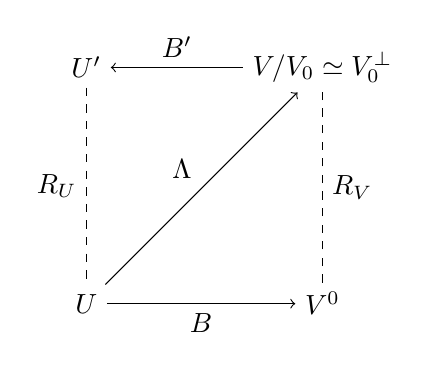
\begin{tikzpicture}
      [auto]
      \node(1) at (0, 0) {$U$};
      \node(2) at (3, 0) {$V^0$};
      \node(3) at (3, 3) {$V/V_0 \simeq V_0^\perp$};
      \node(4) at (0, 3) {$U^\prime$};
      \draw[->](1) --node[below]{$B$} (2);
      \draw[dashed](2) --node[right]{$R_V$} (3);
      \draw[->](3) --node[above]{$B^\prime$} (4);
      \draw[dashed](4) --node[left]{$R_U$} (1);
      \draw[->](1) --node[above left]{$\Lambda$} (3);
  \end{tikzpicture}
\end{center}

其中$V_0 = N(B^\prime)$,$V^0$为$V_0$的零化子空间,限制之后$R_V$仍是等距同构。

现在回过头来,对于自反Banach空间
\begin{center}
  \begin{tikzpicture}
      [auto]
      \node(1) at (0, 0) {$U$};
      \node(2) at (3, 0) {$V^\prime$};
      \node(3) at (3, 3) {$V$};
      \node(4) at (0, 3) {$U^\prime$};
      \node(5) at (-3, 0) {$U^{\prime \prime}$};
      \node(6) at (6, 3) {$V^{\prime \prime}$};
      \draw[->](1) --node[below]{$B$} (2);
      \draw[->](3) --node[above]{$B^\prime$} (4);
      \draw[dashed](2) -- (3);
      \draw[dashed](1) -- (4);
      \draw[->](1) --node[below]{$J_U$} (5);
      \draw[->](3) --node[above]{$J_V$} (6);
      \draw[dashed](4) -- (5);
      \draw[dashed](2) -- (6);
      \draw[<->] (-0.3, 1.5) --node[below]{\scriptsize{Reflexive}} (-1.2, 1.5);
      \draw[<->] (3.3, 1.5) --node[above]{\scriptsize{Reflexive}} (4.2, 1.5);
  \end{tikzpicture}
\end{center}

Conjugate in Banach, Adjoint in Hilbert

对于协调元离散问题:给定$U_{h} \subset U, V_{h} \subset V$,找$u_{h} \in U_{h}$ s.t.
\[
  b(u_{h}, v_{h})=\langle f, v_h\rangle_{V^{\prime} \times V}, \quad \forall v_{h} \in V_{h}
\]

离散问题的适定性. 只需下述离散的inf-sup条件成立
\[
  \text{d. } \qquad \inf_{u_{h} \in U_{h}} \sup _{v_{h} \in V_{h}} \frac{b\left(u_{h}, v_{h}\right)}{\left\|u_{h}\right\|_{U}\left\|v_{h}\right\|_{V}}=\inf_{v_{h} \in V_{h}} \sup _{u_{h} \in U_{h}} \frac{b\left(u_{h}, v_{h}\right)}{\left\|u_{h}\right\|_{U}\left\|v_{h}\right\|_{V}}=\beta_{h}>0 
\]

对于对称情形(Lax-Milgram定理),连续问题的适定性蕴含离散问题的适定性,但是对于非对称情形(Babuška引理)不成立,简单来说有界性和强制性是可以继承得到,但是inf-sup常数限制在小空间上就不一样了,一般来说$\beta_h \le \beta$。

误差估计:若a. + b. + c. + d. 成立,则连续和离散问题的解都是存在唯一的,且有估计
\[
  \left\|u-u_{h}\right\|_{U} \le \left(1+\frac{M}{\beta_{h}}\right) \inf _{w_{h} \in U_{h}}\left\|u-w_{h}\right\|_{U}
\]

引入投影算子$P_h: U \to U_h$ s.t. $b(u, v) = b(P_h u:=u_h, v)$,则有
\[
  \begin{aligned}
    \|u - u_h\|_U &= \|(I - P_h)u\|\\
    &=\|(I - P_h)(u - w_h)\|\\
    &\le \|I - P_h\|_{op} \|u - w_h\|_U\\
    &\le (1 + \|P_h\|_{op}) \inf_{w_h \in U_h} \|u - w_h\|_U
  \end{aligned}
\]

对于Hilbert空间中的投影算子有$\|I - P\|_{op} = \|P\|_{op}$(see Demkowicz's Notes),于是
\[
  \|u - u_h\|_U \le \|P_h\|_{op} \inf_{w_h \in U_h} \|u - w_h\|_U
\]

其中由$\beta_h \|P_h u\|_U = \sup_{v_h \in V_h} \frac{|b(P_h u, v_h)|}{\|v_h\|}= \sup_{v_h \in V_h} \frac{|b(u, v_h)|}{\|v_h\|} \le M \|u\|_U$,故$\|P_h\|_{op} \le \frac{M}{\beta_h}$。

\subsubsection{Brezzi理论}

鞍点问题连续情形:求$u \in V, p \in Q$ s.t.
\[
  \left\{\begin{array}{ll}
    a(u, v)+b(v, p)=\langle f, v\rangle_{V^{\prime} \times V} & \forall v \in V \\
    b(u, q)=\langle g, q\rangle_{Q^{\prime} \times Q} & \forall q \in Q
  \end{array}\right.
\]

其中$a(\cdot, \cdot): V \times V \to \mathbb{R}, b(\cdot, \cdot): V \times Q \to \mathbb{R}$。

\begin{enumerate}[a.]\setcounter{enumi}{4}
  \item $a(v, v) \ge \alpha\|v\|_{V}^{2}, \quad \forall v \in V_{0}$
  
  即$a(\cdot, \cdot)$在$V_0$上强制,故$A$下有界,$A^\prime$商核后下有界。
  \item $\sup _{0 \neq v \in V} \frac{b(v, q)}{\|v\|_{V}} \geq \beta\|q\|_{Q}, \quad \forall q \in Q$
  
  即$B^\prime$下有界,商左边。
\end{enumerate}

则上述连续问题存在唯一解,且有估计
\[
  \|u\|_{V}+\|p\|_{Q} \le C\left(\|f\|_{V^{\prime}}+\|g\|_{Q^{\prime}}\right)
\]

\begin{center}
  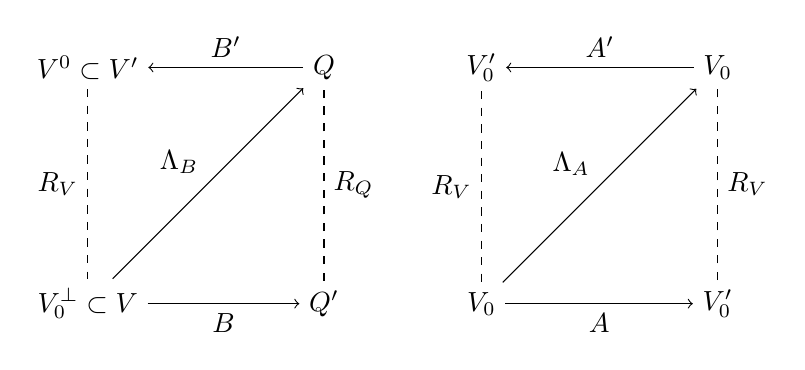
\begin{tikzpicture}
      [auto]
      \node(1) at (0, 0) {$V_0$};
      \node(2) at (3, 0) {$V_0^\prime$};
      \node(3) at (3, 3) {$V_0$};
      \node(4) at (0, 3) {$V_0^\prime$};
      \draw[->](1) --node[below]{$A$} (2);
      \draw[dashed](2) --node[right]{$R_V$} (3);
      \draw[->](3) --node[above]{$A^\prime$} (4);
      \draw[dashed](4) --node[left]{$R_V$} (1);
      \draw[->](1) --node[above left]{$\Lambda_A$} (3);

      \node(5) at (-5, 0) {$V_0^\perp \subset V$};
      \node(6) at (-2, 0) {$Q^\prime$};
      \node(7) at (-2, 3) {$Q$};
      \node(8) at (-5, 3) {$V^0 \subset V^\prime$};
      \draw[->](5) --node[below]{$B$} (6);
      \draw[dashed](6) --node[right]{$R_Q$} (7);
      \draw[->](7) --node[above]{$B^\prime$} (8);
      \draw[dashed](8) --node[left]{$R_V$} (5);
      \draw[->](5) --node[above left]{$\Lambda_B$} (7);
  \end{tikzpicture}
\end{center}

原问题等价于算子方程
\[
  \left\{\begin{array}{ll}
    Au + B^\prime p = f\\
    Bu = g
  \end{array}\right.
\]

pf: 令$V_0 = N(B)$,先由第二个方程的Babuška理论(图1)得到$u_g \in V_0^\perp$以及估计
\[
  \|u_g\|_V \le C\|g\|_{Q^\prime}
\]

再将第一个方程限制在$V_0$上,此时左边第二项消失且$f - Au \in V^0$,由Babuška理论(图2)得到$u_0 = u - u_g \in V_0$以及估计
\[
  \|u_0\|_V \le C\|f - Au_g\|_{V^\prime} \le C\|f\|_{V^\prime} + C\|u\|_V
\]

于是$u = u_g + u_0 \in V$。最后由第一个方程的Babuška理论(图1)得到p以及估计
\[
  \|p\|_Q \le C\|f - Au\|_{V^\prime} \le C\|f\|_{V^\prime} + C\|u\|_V
\]

综上结合$\|u\|_V \le \|u_g\|_V + \|u_0\|_V$可得
\[
  \|u\|_V + \|p\|_Q \le C(\|f\|_{V\prime} + \|g\|_{Q^\prime})
\]

离散问题

给定协调元空间$V_{h} \subset V, Q_{h} \subset Q$,离散问题为:求$u_{h} \in V_{h}, p_{h} \in Q_{h}$ s.t.
\[
  \left\{\begin{array}{ll}
    a\left(u_{h}, v_{h}\right)+b\left(v_{h}, p_{h}\right)=\left\langle f, v_{h}\right\rangle_{V^{\prime} \times V} \quad & \forall v_{h} \in V_{h} \\
    b\left(u_{h}, q_{h}\right)=\left\langle g, q_{h}\right\rangle_{Q^{\prime} \times Q} \quad & \forall q_{h} \in Q_{h}
  \end{array}\right.
\]

若条件e. 和f. 的离散版本$e_h.$ 和$f_h.$(LBB条件)成立,则离散问题解的适定性成立,且有误差估计
\[
  \left\|u-u_{h}\right\|_{v}+\left\|p-p_{h}\right\|_{Q} \leq C\left(\inf _{v_{h} \in V_{h}}\left\|u-v_{h}\right\|_{V}+\inf _{q_{h} \in Q_{h}}\left\|p-q_{h}\right\|_{Q}\right)
\]

pf: 由Galerkin正交性(误差方程)和离散问题解的适定性,见ppt FEM-10 p2。

对于离散问题可以把双线性泛函看成二次型$b_h(u_h, v_h) = u_h^T B v_h$,此时验证LBB条件即估计矩阵B的最小/最大特征值,一般来说这是困难的,于是引入LBB条件的一个充分条件,即Fortin准则。

\begin{thm}
  (Fortin准则)若双线性泛函$b: V \times Q \to \mathbb{R}$满足inf-sup条件,且对于协调元空间$V_h, Q_h$存在有界线性算子$\Pi_h: V \to V_h$ s.t.
  \[
    \begin{aligned}
      b(\Pi_h v, q_h) = b(v, q_h),& \quad \forall q_h \in Q_h\\
      \|\Pi_h v\|_V \le \|v\|_V,& \quad \forall v \in V
    \end{aligned}
  \]

  其中C与h无关(由$C \sim \frac{1}{\beta_h}$,说明离散inf-sup常数$\beta_h$与h无关),则LBB条件成立
\end{thm}

pf:
\[
  \begin{aligned}
    \beta\left\|q_{h}\right\|_{Q} & \leq \sup _{v \in V} \frac{b\left(v, q_{h}\right)}{\|v\|_{V}}=\sup _{v \in V} \frac{b\left(\Pi_{h} v, q_{h}\right)}{\|v\|_{V}} \\
    & \le C \sup _{v \in V} \frac{b\left(\Pi_{h} v, q_{h}\right)}{\left\|\Pi_{h} v\right\|_{V}} \leq C \sup _{v_{h} \in V_{h}} \frac{b\left(v_{h}, q_{h}\right)}{\left\|v_{h}\right\|_{V}}
  \end{aligned}
\]

-----Poisson问题
\[
  \begin{array}{l}
    V = H(\operatorname{div}, \Omega), \quad Q = L^2(\Omega), \quad V_0 = N(\operatorname{div})\\
    a(\undertilde{p}, \undertilde{q})=\int_{\Omega} \undertilde{p} \cdot \undertilde{q} dx, \quad b(\undertilde{q}, v)=\int_{\Omega} \operatorname{div} \undertilde{q} v dx
  \end{array}
\]

验证Brezzi理论条件:
\begin{enumerate}
  \item 有界性即Cauchy-Schwarz不等式。
  \item e. $a(\undertilde{p}, \undertilde{p}) = \sum_i\|p_i\|_{0, \Omega}^2 = \|\undertilde{p}\|_{0, \Omega}^2 = \|\undertilde{p}\|_{\operatorname{div}, \Omega}^2, \forall \undertilde{p} \in V_0$($\|\undertilde{p}\|_{\operatorname{div}, \Omega} = \|\undertilde{p}\|_{0, \Omega} + \|\operatorname{div} \undertilde{p}\|_{0, \Omega}$)
  \item f. 利用Poisson方程构造性证明:(构造性就是找一个成立)
  
  考虑Dirichlet边值条件的Poisson问题$\left\{\begin{array}{l}
    -\Delta \phi=q \\
    \phi|_{\partial \Omega}=0
  \end{array}\right.$,取$\undertilde{p} = - \nabla \phi \in H(\operatorname{div}, \Omega)$,则
  \[
    \begin{aligned}
      &(\operatorname{div} \undertilde{p}, q)=(-\operatorname{div} \nabla \phi, q)=(q, q)=\|q\|_{0, \Omega}^{2}\\
      &\|\undertilde{p}\|_{\operatorname{div}, \Omega}^{2}=\|\undertilde{p}\|_{0, \Omega}^{2}+\|\operatorname{div} \undertilde{p}\|_{0, \Omega}^{2}=\|\nabla \phi\|_{0, \Omega}^{2}+\|q\|_{0, \Omega}^{2} \leq C\|q\|_{0, \Omega}^{2} 
    \end{aligned}
  \]

  最后一个不等号是由正则性$\|\phi\|_{1, \Omega} \leq C\|g\|_{-1, \Omega} \leq C\|q\|_{0, \Omega}$。于是
  \[
    \sup_{0 \neq \undertilde{p} \in V} \frac{(\operatorname{div} \undertilde{p}, q)}{\|\undertilde{p}\|_{\operatorname{div}, \Omega}} \ge \frac{\|q\|_{0, \Omega}^2}{\sqrt{C}\|q\|_{0, \Omega}} = \frac{1}{\sqrt{C}}\|q\|_{0, \Omega}, \quad \forall q \in Q
  \]
\end{enumerate}

-----Stokes问题
\[
  \begin{array}{l}
    V = \left(H_0^1(\Omega)\right)^d, \quad Q = L_0^2(\Omega), \quad V_0 = N(\operatorname{div})\\
    a(\undertilde{u}, \undertilde{v})=\int_{\Omega} \nabla \undertilde{u}: \nabla \undertilde{v} dx, \quad b(\undertilde{v}, q)=-\int_{\Omega} \operatorname{div} \undertilde{v} q dx
  \end{array}
\]

验证Brezzi理论条件
\begin{enumerate}
  \item 有界性
  \item e. 由Poincaré不等式,$a(\undertilde{u}, \undertilde{u}) = \|\nabla \undertilde{u}\|_0 \ge \|u\|_1, \forall \undertilde{u} \in V$
  \item f. 考虑二维区域且边界是凸的或充分光滑。构造性证明:
  
  注意到$\operatorname{div}: V \to L_0^2(\Omega)$是满的,$\forall q \in L_0^2(\Omega), \exists \undertilde{v} \in V, -\operatorname{div} \undertilde{v} = q$,再设$\undertilde{v} = \operatorname{grad}\phi, \phi \in H^1(\Omega)$,于是$-\Delta \phi = q$。

  要想$\undertilde{v} = \nabla \phi \in V = (H_0^1(\Omega))^2$,需要$\nabla \phi \cdot \nu|_{\partial \Omega} = \nabla \phi \cdot \tau|_{\partial \Omega} = 0$,第一个条件直接加在$\phi$上,可得Neumann边值条件的Poisson问题$\left\{\begin{array}{l}
    -\Delta \phi=q \\
    \nabla \phi \cdot \nu|_{\partial \Omega}=0
  \end{array}\right.$。再去修正切向导数,为了不破坏Poisson问题,设$\left\{\begin{array}{l}
    \undertilde{w} = \operatorname{curl} \psi\\
    \psi|_{\partial \Omega} = 0\\
    \nabla \psi \cdot \nu|_{\partial \Omega} = - \nabla \phi \cdot \nu|_{\partial \Omega}
  \end{array}\right.$。故$\undertilde{u} = \undertilde{v} + \undertilde{w} \in V, \operatorname{div}\undertilde{u} = q$,由$\phi, \psi \in H^2(\Omega)$可得正则性$\|\undertilde{v}\|_{1, \Omega} \le C\|q\|_{0, \Omega}$以及$\|\undertilde{w}\|_{1, \Omega} \le C\|v\|_{0, \Omega}$。于是
  \[
    \sup_{0 \neq \undertilde{p} \in V} \frac{(\operatorname{div} \undertilde{p}, q)}{\|\undertilde{p}\|_{1, \Omega}} \ge \frac{(\operatorname{div} \undertilde{u}, q)}{\|\undertilde{u}\|_{1, \Omega}} \ge C\|q\|_{0, \Omega}, \quad \forall q \in Q
  \]
  



  
  一般区域上的结论和正则性见Girault, Raviart。
\end{enumerate}

----- Stokes问题的有限元离散

$P_2 - P_0$元
\[
  \begin{array}{l}
    S_{h}=\left\{v_{h} \in H^{1}(\Omega) \mid v_{h}|_{K} \in P_{2}(K), \forall K \in \mathcal{T}_{h}\right\} \text{ (Lagrange二次元)}\\
    M_{h}=\left\{q_{h} \in L^{2}(\Omega) \mid q_{h}|_{K} \in P_{0}(K), \forall K \in \mathcal{T}_{h}\right\} \text{ (分片常数)}\\
    V_{h}=\left(S_{h} \cap H_{0}^{1}(\Omega)\right)^{2}, Q_{h}=M_{h} \cap L_{0}^{2}(\Omega)
  \end{array} 
\]

定义$\Pi_h^1: H_0^1(\Omega) \to S_h \cap H_0^1(\Omega)$为Lagrange二次元的Scott-Zhang插值,则有插值误差估计
\[
  \left\|\undertilde{v}-\Pi_{h}^{1} \undertilde{v}\right\|_{0, K}+h_{K}|\undertilde{v}-\Pi_{h}^{1} \undertilde{v}|_{1, K} \le h_{K}|\undertilde{v}|_{1, \omega_{K}}
\]

但是$\Pi_h^1$不是可交换的,即不满足Fortin准则1. ,于是引入插值$\Pi_h^2$进行修正
\[
  \left\{\begin{array}{l}
    \Pi_{h}^{2} v\left(a_{i}\right)=0, \quad i = 1, 2, 3 \\
    \int_{e_{i}} \Pi_{h}^{2} v \mathrm{ds}=\int_{e_{i}} v \mathrm{ds}, \quad i = 1, 2, 3
  \end{array}\right.
\]

若有可交换性$b(v - \Pi_h v, q_h) = 0, \forall q_h \in Q_h$,则$\sum_K \int_K \operatorname{div}(v - \Pi_h v) q_h dx = \sum_K q_h \int_K \operatorname{div}(v - \Pi_h v) dx = 0$,故只需要$\int_K \operatorname{div}(v - \Pi_h v) dx = 0, \forall K$,其中最后一个等号是因为$q_h \in Q_h$是分片常数。

其有界性(HW 10.3)
\[
  \left\|\Pi_{h}^{2} \undertilde{v}\right\|_{0, K} \le C\left(\|\undertilde{v}\|_{0, K}+h_{K}|\undertilde{v}|_{1, K}\right)
\]

构造Fortin插值$\Pi_h$ s.t. $I - \Pi_h = (I - \Pi_h^2)(I - \Pi_h^1)$。把$(I - \Pi_h^1)v$看成一个整体,则$\Pi_h$是可交换的。
\[
  \begin{aligned}
    \left|\Pi_{h} \undertilde{v}\right|_{1, \Omega}^{2} & \le \left|\Pi_{h}^{1} \undertilde{v}\right|_{1, \Omega}^{2}+\left|\Pi_{h}^{2}\left(\undertilde{v}-\Pi_{h}^{1} \undertilde{v}\right)\right|_{1, \Omega}^{2}\\
    & \le C|\undertilde{v}|_{1, \Omega}^{2}+C \sum_{K \in \mathcal{T}_{h}} h_{K}^{-2}\left\|\Pi_{h}^{2}\left(\undertilde{v}-\Pi_{h}^{1} \undertilde{v}\right)\right\|_{1, K}^{2}\\
    & \le C|\undertilde{v}|_{1, \Omega}^{2}+C \sum_{K \in \mathcal{T}_{h}}\left(h_{K}^{-2}\left\|\undertilde{v}-\Pi_{h}^{1} \undertilde{v}\right\|_{0, K}^{2}+\left|\undertilde{v}-\Pi_{h}^{1} \undertilde{v}\right|_{1, K}^{2}\right)\\
    & \le C|\undertilde{v}|_{1, \Omega}^{2}
  \end{aligned}
\]

分别是:三角不等式,Scott-Zhang插值有界性和逆估计,$\Pi_h^2$有界性,Scott-Zhang插值误差估计。

最后有插值误差估计
\[
  \left\|\undertilde{u}-\undertilde{u}_{h}\right\|_{1, \Omega}+\left\|p-p_{h}\right\|_{0, \Omega} \leq C\left(\inf_{\undertilde{v}_{h} \in V_{h}}\left\|\undertilde{u}-\undertilde{v}_{h}\right\|_{1, \Omega}+\inf _{q_{h} \in Q_{h}}\left\|p-q_{h}\right\|_{0, \Omega}\right)
\]

若$\undertilde{u} \in\left(H^{2}(\Omega)\right)^{2}, p \in H^{1}(\Omega)$,则由估计插值误差估计可得
\[
  \left\|\undertilde{u}-\undertilde{u}_{h}\right\|_{1, \Omega}+\left\|p-p_{h}\right\|_{0, \Omega} \leq C\left(h^{2}|\undertilde{u}|_{2, \Omega}+h|p|_{1, \Omega}\right)
\]

h的阶数出自Lagrange二次元的$H^1$误差估计和分片常数的$L^2$误差估计。

\section{后验误差估计}

\newpage

\section{一些}
一些映射:
\begin{enumerate}
  \item 插值算子:$\Pi_K: C^\ell(K) \to W^{m, p}(K), \Pi_K u = \sum_i N_i(u) \Phi_i$
  \item 投影算子:$P_m: W^{m, p}(\Omega) \to P_m(\Omega)$
\end{enumerate}

一些不等式:
\begin{enumerate}
  \item 1. Young不等式: $a b \le \frac{1}{p} a^{p}+\frac{1}{q} b^{q}$. (a, b $\ge$ 0 in case you dont know)

  2. Holder不等式: $\|f \cdot g\|_{0, 1, \Omega} \le\|f\|_{0, p, \Omega}\|g\|_{0, q, \Omega}$. Proof by Young不等式.
  
  3. Minkowski不等式: $\|f+g\|_{0, p, \Omega} \le\|f\|_{0, p, \Omega}+\|g\|_{0, p, \Omega}$.
  \item Sobolev空间中的范数等价定理
  \begin{enumerate}
    \item Poincaré-Friedrichs不等式:
    \[
      \|v\|_{m, \Omega} \le C_{1}|v|_{m, \Omega}, \forall v \in H_{0}^{m}(\Omega).
    \]
    \item Poincaré不等式:
    \[
      \|v\|_{m, \Omega}^{2} \le C_{2}\left(|v|_{m, \Omega}^{2}+\sum_{|\alpha|<m}\left(\int_{\Omega} \partial^{\alpha} v dx\right)^{2}\right), \forall v \in H^{m}(\Omega).
    \]
    m = 1时:
    \[
      \|v\|_{1, \Omega}^{2} \le C_{2}\left(|v|_{1, \Omega}^{2}+\left(\int_{\Omega} v dx\right)^{2}\right), \forall v \in H^{1}(\Omega).
    \]
  \end{enumerate}
  \item Poincaré不等式:
  \[
    \left\|u-(u)_{U}\right\|_{0, p, U} \le C\|D u\|_{0, p, U} = C\sum_{i} \|\partial_i u\|_{0, p, U}, \forall u \in W^{1, p}(U).
  \]
\end{enumerate}

一些估计:
\begin{enumerate}[]
  \item 几何估计:$\|B\| \le \frac{h_{K}}{\rho_{\widehat{K}}},|\operatorname{det} B| \le C\left(\frac{h_{K}}{\rho_{\widehat{K}}}\right)^{n}$。
  \item 单元估计:$|\widehat{v}|_{m, p, \widehat{K}} \le C\|B\|^{m}|\operatorname{det} B|^{-1 / p}|v|_{m, p, K}$。
  \item 单元边界估计:$\|\widehat{v}\|_{0, p, \partial \widehat{K}} \le C\|B\|^{1 / p}|\operatorname{det} B|^{-1 / p}\|v\|_{0, p, \partial K}$。
  \item Verfürth投影估计:$\left\|u-P_{k} u\right\|_{k+1, p, \Omega} \le C(m, n, \gamma)|u|_{k+1, p, \Omega}$。
  \item 局部插值误差估计:$\|v - \Pi_K v\|_{i, p, K} \le C h^{m - i} \|v\|_{m, p, K}$
  \item 整体插值误差估计:$\left(\sum_{K \in \mathcal{T}_{h}}\left\|v-\Pi_{K} v\right\|_{s, p, K}^{p}\right)^{1 / p} \le C h^{m-s}|v|_{m, p, \Omega}$。
  \item 局部逆估计:$\|v\|_{\ell, p, K} \le C h^{m-\ell+n / p-n / q}\|v\|_{m, q, K}$。
  \item 整体逆估计:
\end{enumerate}

一些题目:

证明基本不等式

证明空间完备性

求弱形式

证明弱解在一定正则性下就是古典解





一些技巧:

空间稠密性

反证法

算子角度

一些问题:285

flag
